%% 
%% Copyright 2019-2020 Elsevier Ltd
%% 
%% This file is part of the 'CAS Bundle'.
%% --------------------------------------
%% 
%% It may be distributed under the conditions of the LaTeX Project Public
%% License, either version 1.2 of this license or (at your option) any
%% later version.  The latest version of this license is in
%%    http://www.latex-project.org/lppl.txt
%% and version 1.2 or later is part of all distributions of LaTeX
%% version 1999/12/01 or later.
%% 
%% The list of all files belonging to the 'CAS Bundle' is
%% given in the file `manifest.txt'.
%% 
%% Template article for cas-sc documentclass for 
%% double column output.

% \documentclass[a4paper,fleqn,longmktitle]{cas-sc}
\documentclass[a4paper]{cas-sc}
% \documentclass{article}
% \usepackage[numbers]{natbib}
\usepackage[authoryear]{natbib}

% \usepackage[authoryear,longnamesfirst]{natbib}

\usepackage{threeparttable}
% \usepackage[section]{placeins}
\usepackage{afterpage}
% \usepackage[disable]{endfloat}
\usepackage{amsmath}
\usepackage{ntheorem}
\newtheorem{theorem}{Theorem}
\newtheorem{lemma}[theorem]{Lemma}
\newtheorem*{proof}{Proof}
\newtheorem{remark}[theorem]{Remark}
\newtheorem{defi}[theorem]{Definition}
\newtheorem{property}[theorem]{Property}
\newtheorem{corollary}[theorem]{Corollary}
%%%Author definitions
\def\tsc#1{\csdef{#1}{\textsc{\lowercase{#1}}\xspace}}
\tsc{WGM}
\tsc{QE}
\tsc{EP}
\tsc{PMS}
\tsc{BEC}
\tsc{DE}
%%%

% Uncomment and use as if needed
%\newtheorem{theorem}{Theorem}
%\newtheorem{lemma}[theorem]{Lemma}
%\newdefinition{rmk}{Remark}
%\newproof{pf}{Proof}
%\newproof{pot}{Proof of Theorem \ref{thm}}

\begin{document}
\let\WriteBookmarks\relax
\def\floatpagepagefraction{1}
\def\textpagefraction{.001}


% Short author
\shortauthors{Tiancheng Ruan et~al.}
\shorttitle{}

% Main title of the paper
\title [mode = title]{A general representation of the heterogeneous Leader-based Connected Automated Vehicle platoon and stability analyses considering multiple delays}
% Title footnote mark
% eg: \tnotemark[1]
% \tnotemark[1,2]

% Title footnote 1.
% eg: \tnotetext[1]{Title footnote text}
% \tnotetext[<tnote number>]{<tnote text>} 
% \tnotetext[1]{This document is the results of the research
%    project funded by the National Science Foundation.}

% \tnotetext[2]{The second title footnote which is a longer text matter
%    to fill through the whole text width and overflow into
%    another line in the footnotes area of the first page.}


% First author
%
% Options: Use if required
% eg: \author[1,3]{Author Name}[type=editor,
%       style=chinese,
%       auid=000,
%       bioid=1,
%       prefix=Sir,
%       orcid=0000-0000-0000-0000,
%       facebook=<facebook id>,
%       twitter=<twitter id>,
%       linkedin=<linkedin id>,
%       gplus=<gplus id>]
\author[1,2,3]{Tiancheng Ruan}[style=chinese]
\ead{ruantiancheng@seu.edu.cn}
\credit{Conceptualization of this study, Methodology,Writing - Original draft preparation,Resources, Software}

\author[1,2,3]{Hao Wang}[style=chinese]
% Corresponding author indication
\cormark[1]

% % Footnote of the first author
% \fnmark[1]

% Email id of the first author
\ead{haowang@seu.edu.cn}

% % URL of the first author
% \ead[url]{www.cvr.cc, cvr@sayahna.org}

%  Credit authorship
\credit{ Formal analysis,Funding acquisition,Supervision,Writing - review \& editing}

% Address/affiliation
\affiliation[1]{organization={Jiangsu Key Laboratory of Urban ITS, Southeast University},
  addressline={2 Si Pai Lou},
  city={Nanjing},
  % citysep={}, % Uncomment if no comma needed between city and postcode
  postcode={210096},
  % state={},
  country={P.R. China}}

\affiliation[2]{organization={Jiangsu Province Collaborative Innovation Center of Modern Urban Traffic Technologies},
  addressline={2 Si Pai Lou},
  city={Nanjing},
  % citysep={}, % Uncomment if no comma needed between city and postcode
  postcode={210096},
  % state={},
  country={P.R. China}}
\affiliation[3]{organization={School of Transportation, Southeast University},
  addressline={2 Si Pai Lou},
  city={Nanjing},
  % citysep={}, % Uncomment if no comma needed between city and postcode
  postcode={210096},
  % state={},
  country={P.R. China}}
% Second author


% Third author
\author[1,2,3]{Linjie Zhou}[style=chinese]
% \fnmark[2]
\ead{220193107@seu.edu.cn}
% \ead[URL]{www.sayahna.org}
\credit{Data curation,Investigation}



% Fourth author
% \author%
% [4]

\author[1,2,3]{Yujia Chen}[style=chinese]
% \fnmark[2]
\ead{chenyujia@seu.edu.cn}
% \ead[URL]{www.sayahna.org}
\credit{Writing - Original draft preparation}

\author[1,2,3]{Changyin Dong}[style=chinese]
% \fnmark[2]
\ead{dongcy@seu.edu.cn}
% \ead[URL]{www.sayahna.org}
\credit{Formal analysis,Funding acquisition}
% \affiliation[4]{organization={MOE Key Laboratory for UrbanTransportation Complex Systems Theory and Technology, Beijing Jiaotong University},
%     city={Beijing},
%     % citysep={}, % Uncomment if no comma needed between city and postcode
%     postcode={100044}, 
%     % state={},
%     country={P.R. China}}
% \affiliation[5]{organizati on={State Key Laboratory of Fire Science and School of Engineering Science, University of Science and Technology of China},
%     city={Hefei},
%     % citysep={}, % Uncomment if no comma needed between city and postcode
%     postcode={230026}, 
%     % state={},
%     country={P.R. China}}



% Corresponding author text
\cortext[cor1]{Corresponding author}

% Footnote text
% \fntext[fn1]{This is the first author footnote. but is common to third
%   author as well.}
% \fntext[fn2]{Another author footnote, this is a very long footnote and
%   it should be a really long footnote. But this footnote is not yet
%   sufficiently long enough to make two lines of footnote text.}

% For a title note without a number/mark
% \nonumnote{This note has no numbers. In this work we demonstrate $a_b$
%   the formation Y\_1 of a new type of polariton on the interface
%   between a cuprous oxide slab and a polystyrene micro-sphere placed
%   on the slab.
%   }

% Here goes the abstract
\begin{abstract}
  Urged by the potential of Connected Automated Vehicles (CAVs), research has recently focused on studying their benefits on safety, emissions, and capacity. However, in most works, the CAV has been studied in isolation, and there is a lack of in-depth research on stability conditions. Therefore, this paper proposes a general representation of the heterogeneous Leader-based CAV platoon considering multiple delays. Moreover, a novel and more unconservative stability condition of the CAV platoon is derived under the general representation proposed based on the Lyapunov-Krasovskii Stability Theorem and Bessel-Legendre inequalities. Furthermore, a comprehensive performance evaluation analysis of the four typical Leader-based information flow topologies (IFTs) is conducted to test tracking performance and safety conditions by numerical analyses. The results show that the CACC platoon has superior tracking performance in various scenarios if stability is guaranteed. Moreover, bi-directional communication that receives more information in most cases enables better safety condition for hard braking maneuver situations.
\end{abstract}

% Use if graphical abstract is present
% \begin{graphicalabstract}
% 
\includegraphics{figs/grabs.pdf}
% \end{graphicalabstract}

% Research highlights
\begin{highlights}
  \item A general representation of the heterogeneous Leader-based CAV platoon as a state delay system is proposed considering multiple delays.
  \item A novel and more unconservative stability condition of the CAV platoon is derived under the general representation proposed.
  \item A comprehensive performance evaluation analysis of the four typical Leader-based IFTs is performed in a variety of scenarios.

\end{highlights}

% Keywords
% Each keyword is seperated by \sep
\begin{keywords}
  Connected Automated Vehicle (CAV) \sep CAV platoon \sep General modeling of CAV platoon \sep Stability analyses \sep State delay system
\end{keywords}


\maketitle

\section{Introduction}
\label{Section 1}

Since the invention of the automobile over a century ago, automotive engineers have been committed to providing safer and more comfortable services. However, traffic problems such as traffic congestion, traffic accidents, and pollutant emissions have become increasingly prominent in past decades with the development of technology \citep{Schrank2012,Jin2016}. Traditional traffic engineering relies on external measures such as traffic management, traffic control, and so forth to improve traffic capacity and service levels. Nevertheless, these methods are inherently inefficient to satisfy the ever-growing traffic demand. By studying the dynamic and static characteristics of traffic flow, it can be found that the extensive heterogeneity of human factors causes the uncertainty in road traffic \citep{Zhong2020,Ye2018,Arem2016,Yu2021}, which worsens traffic flow stability and restricts capacity.

Fortunately, Automated Vehicle (AV) stands out as a promising enabler and has gained significant popularity in academia and the automotive industry in recent years. It tracks the predecessor based on on-board sensory devices to maintain a constant gap/time gap and becomes increasingly available as standard equipment in modern commercial vehicles with the market penetration rate (MPR) increasing \citep{Wilson2011}. Despite its relatively short history, plentiful research has demonstrated its advantages regarding safety, emissions, and capacity over human drivers \citep{Wang2019,Sarker2019,Dey2015}.

However, AV is inadequate to fully liberate the potential of autonomous driving. Thanks to the development of Cellular vehicle-to-everything (C-V2X) and wireless communication technology, Connected Automated Vehicle (CAV) emerges by using Vehicle-to-Infrastructure (V2I) / Vehicle-to-Vehicle (V2V) communication to further improve safety and capacity. CAV has the potential to achieve more complex controls compared to AV due to its ability to obtain more adequate and timely information through communication \citep{Navas2019,Ruan2021,Zhou2021}. Moreover, CAVs can achieve system optimization rather than user equilibrium by forming a CAV platoon, which can maximize the gain brought by CAVs compared to traditional transportation \citep{Firooznia2017,Hu2021}.

There has been extensive research on CAV, including exploring its gain for capacity \citep{Ghiasi2017,Chang2020}, stability \citep{Zhou2019,Montanino2021}, eco-driving \citep{Qin2018,Ruan2022}, and designing control strategies of CAVs \citep{Zhu2019,Chen2021}. However, the modeling object in existing research is only one CAV \citep{Wei2017,Navas2016,Milanes2014a} or a specific information flow topology (IFT) for specific research goals \citep{Wang2021,Chin2015}, which ignores the needs and potential of the CAV platoon as a modeling object. Besides, as for the stability analyses, some studies focus only on string stability and ignore stability by assuming that the CAV platoon is local stable \citep{Studli2017,Wang2018a}, while others study the local stability of one CAV \citep{Zhou2019a,Monteil2019}. The former strategy is correct to a certain extent if the communication delay is ignored. However, the communication delay cannot be ignored in practice which means it is necessary to consider the communication delay when exploring the stability condition. As for the latter strategy, the stability condition is derived based on Routh-Hurwitz stability criterion or Lyapunov second method in most research. However, the results obtained based on this method are conservative and underperformed in the state delay system. Therefore, modeling the generalized CAV platoon and developing a novel stability approach with less conservativeness need to be conducted for further analyses.

To fill the gap, this paper proposes a general representation of the heterogeneous Leader-based CAV platoon and a stability condition of the CAV platoon based on the general representation. To sum up, the main contribution of the paper is threefold:
\begin{enumerate}
  \item A general representation of the heterogeneous Leader-based CAV platoon as a state delay system is proposed considering multiple delays.
  \item A novel and more unconservative stability condition of the CAV platoon is derived under the general representation proposed based on the Lyapunov-Krasovskii Stability Theorem and Bessel-Legendre inequalities.
  \item A comprehensive performance evaluation analysis of the four typical Leader-based IFTs is performed to reveal tracking performance, transient response, and safety conditions in a variety of scenarios.
\end{enumerate}

The remainder of the paper is outlined as follows: Section~\ref{Section 2} introduces the mathematical background, including graph theory and primary matrix inequalities. Section~\ref{Section 3} presents the problem statement and a general representation of the heterogeneous Leader-based CAV platoon. Corresponding stability analyses and the derivation of stability conditions based on the Lyapunov-Krasovskii Stability Theorem are carried out in Section~\ref{Section 4}. Section~\ref{Section 5} proposes a comprehensive performance evaluation analysis of the four typical Leader-based IFTs. We summarize the study in Section~\ref{Section 6}.

\textbf{Notations:} Throughout the paper ${\mathbb{R}^n}$ denotes the n-dimensional Euclidean space with Euclidian norm $| \cdot |$  while the set of all $m \times n$ real matrices is denoted by ${\mathbb{R}^{m \times n}}$ . The sets $ {\mathbb{S}_n} $ and $\mathbb{S}_n^ + $ mean the set of symmetric and symmetric positive definite matrices of ${\mathbb{R}^{n \times n}}$, respectively. The transpose of a vector or a matrix $A $ is denoted by ${A^T} $. The symmetric matrix $\left[ {\begin{array}{*{20}{c}}
          A & B \\
          * & C
        \end{array}} \right]$ denotes $\left[ {\begin{array}{*{20}{c}}
          A       & B \\
          {{B^T}} & C
        \end{array}} \right]$. Besides, for any square matrix $ A \in {\mathbb{R}^{n \times n}}$, we define $ He\left( A \right) = A + {A^T}$. ${I_n} $ defines the identity matrix of $ n \times n $ dimension while ${0_{m,n}} $ stands for the zero matrix of $ m \times n$ dimension. For any matrix $A \in {\mathbb{R}^{n \times n}} $, the notation $ A \succ 0$ denotes that $A $ is symmetric and positive definite. The set of continuous functions from an interval $\left[ { - h,0} \right] \subset \mathbb{R}$ to ${\mathbb{R}^n}$ which are, consequently, square integrable is demoted as Banach space $\mathcal{C}\left( {\left[ { - h,0} \right],{\mathbb{R}^n}} \right)$. For any function $f \in \mathcal{C}$, the uniform norm $|f{|_h}$ refers to $\mathop {\sup }\limits_{\theta  \in [ - h,0]} |f(\theta )|$. $diag\left\{ {{a_1},{a_2}, \cdots ,{a_n}} \right\}$ stands for the diagonal matrix $\left[ {\begin{array}{*{20}{c}}
          {{a_1}} & 0      & 0       \\
          0       & \ddots & 0       \\
          0       & 0      & {{a_n}}
        \end{array}} \right]$ whose diagonal elements starting at the upper left corner are ${a_1},{a_2}, \cdots ,{a_n}$. The notation $\left( {\begin{array}{*{20}{c}}
      k \\
      l
    \end{array}} \right)$ defines the binomial coefficients given by $\frac{{k!}}{{\left( {k - l} \right)!l!}}$. Moreover, $\left\langle {f,g} \right\rangle $ presents the inner product for $\forall f,g \in \mathcal{C}$.\\
Let $A \in {\mathbb{R}^{m \times n}}$ and $B \in {\mathbb{R}^{p \times q}}$ , then  $A \otimes B$ is the Kronecker product of $A$ and $B$:
\begin{equation*}
  A \otimes B = \left[ {\begin{array}{*{20}{c}}
          {{a_{11}}B} & \cdots & {{a_{1n}}B} \\
          \vdots      & \ddots & \vdots      \\
          {{a_{m1}}B} & \cdots & {{a_{mn}}B}
        \end{array}} \right] \in {\mathbb{R}^{mp \times nq}}
\end{equation*}
Let $C \in {\mathbb{R}^{m \times n}} $ and $D \in {\mathbb{R}^{m \times n}} $, then $C \circ D$ is the Hadamard product of $C$ and $D$:
\begin{equation*}
  C \circ D = \left[ {\begin{array}{*{20}{c}}
          {{c_{11}}{d_{11}}} & \cdots & {{c_{1n}}{d_{1n}}} \\
          \vdots             & \ddots & \vdots             \\
          {{c_{m1}}{d_{m1}}} & \cdots & {{c_{mn}}{d_{mn}}}
        \end{array}} \right] \in {\mathbb{R}^{m \times n}}
\end{equation*}


\section{Mathematical preliminaries}
\label{Section 2}
Before providing analyses, we introduce some primary mathematical preliminaries first .

\subsection{Network model}
\label{Section 2.1}

By regarding each vehicle in the platoon as a node and intervehicle communication as an edge, the information flow topology (IFT) among the platoon can be modeled as a weighted directed graph (digraph) $ \mathcal{G} = \left\{ {\mathcal{V},\mathcal{E},\mathcal{A}} \right\}$, in which $\mathcal{V} = \left\{ {1,2, \cdots ,n} \right\}$ is the set of nodes and $\mathcal{E} \subseteq \mathcal{V} \times \mathcal{V} $ is the set of edges. Besides, the weighted adjacent matrix with nonnegative elements is defined as $\mathcal{A} = {[{a_{ij}}]_{n \times n}}$ with ${a_{ii}} = 0$ which denotes that the self-edges $\left( {i,i} \right)$ is not allowed unless indicated otherwise. The edge $\left( {i,j} \right)$ in $\mathcal{E}$ means the vehicle $i$ can communicate with vehicle $j$ associated with weighted ${a_{ij}}$. Defining the degree matrix of $\mathcal{G}$ as $\mathcal{D} = diag\left\{ {{d_1},{d_2}, \cdots ,{d_n}} \right\}$, with ${d_i} = \sum\limits_{j \in \mathcal{V}} {{a_{ij}}} $. Therefore, the Laplacian matrix $\mathcal{L}$ of the weighted digraph $\mathcal{G}$ can be defined as $\mathcal{L} = \mathcal{D} - \mathcal{A}$. It should be noted that the heterogeneity referred to herein is the heterogeneity of the control gains employed by different CAVs.

\subsection{Stability of state delay system}
\label{Section 2.2}

Consider a linear state delay system described by:
\begin{equation}
  \left\{ {\begin{array}{*{20}{l}}
        {\dot x(t) = Ax(t) + {A_d}x(t - h),} & {\forall t \geqslant 0,}  \\
        {x(t) = \phi (t),}                   & {\forall t \in [ - h,0],}
      \end{array}} \right.
  \label{eq1}
\end{equation}
where $x(t) \in {\mathbb{R}^n}$ is the state vector; $ \phi $ stands for the initial conditions; $A $ and $A_d $ are constant matrixes; $ h$ denotes the known constant time delay.

In the context of the stability analysis of state delay systems, the Lyapunov-Krasovskii Stability Theorem is a well-known approach extending the second Lyapunov method dedicated to stability analysis \citep{Gu2003}. It includes the "energy" functionals that are positive definite, and decrease along the trajectories of the system. The Lyapunov-Krasovskii theorem is stated below:
\begin{lemma}
  \label{lemma1}
  (Lyapunov-Krasovskii Stability Theorem) \citep{Gu2009}. Given system (\ref{eq1}), suppose that $f$ maps $\mathbb{R} \times  $(bounded sets in ${\mathbb{R}^n} \times \mathcal{C} $) into bounded sets in ${\mathbb{R}^n} $, and that $u,v,w:{\mathbb{R}_ + } \to {\mathbb{R}_ + } $ are continuous nondecreasing functions, where additionally $u(s) $ and $v(s) $ are positive for $s > 0 $, and $u(0) = v(0) = 0 $. If there exists a functional $V:\mathbb{R} \times {\mathbb{R}^n} \times \mathcal{C} \to \mathbb{R} $ such that
  \begin{equation}
    \left\{ \begin{gathered}
      u(|\phi \left( 0 \right)|) \leqslant V(t,\phi ) \leqslant v(|\phi {|_h}) \hfill \\
      \dot V(t,\phi ) \leqslant  - w(|\phi \left( 0 \right)|) \hfill \\
    \end{gathered}  \right.
  \end{equation}
  Then the trivial solution of the system (\ref{eq1}) is uniformly stable. If $w(s) > 0 $ for $s > 0 $, then it is uniformly asymptotically stable. If, in addition, $\mathop {\lim }\limits_{s \to \infty } u(s) =  + \infty  $, then it is globally uniformly asymptotically stable. Such a functional $V $ is called a Lyapunov-Krasovskii functional (LKF).
\end{lemma}

\begin{defi}
  (Legendre polynomials). The Legendre polynomials considered over the interval $[ - h,0]$ are defined by:
  \begin{equation}
    {\mathcal{L}_k}(u) = {( - 1)^k}\sum\limits_{l = 0}^K {p_l^k} {\left( {\frac{{u + h}}{h}} \right)^l},\quad \quad \forall k \in \mathbb{N}
  \end{equation}
  where $p_l^k = {( - 1)^l}\left( {\begin{array}{*{20}{l}}
        k \\
        l
      \end{array}} \right)\left( {\begin{array}{*{20}{c}}
        {k + l} \\
        l
      \end{array}} \right)$.
\end{defi}

These Legendre polynomials satisfy the following properties:
\begin{property}

  \textit{P3.1} Orthogonality:
  \begin{equation}
    \int_{ - h}^0 {{\mathcal{L}_k}} (u){\mathcal{L}_l}(u){\text{d}}u = \left\{ {\begin{array}{*{20}{l}}
          {0,}                  & {k \ne l} \\
          {\frac{h}{{2k + 1}},} & {k = l}
        \end{array}} \right.\quad \quad \forall (k,l) \in {\mathbb{N}^2}
    \label{p3.1}
  \end{equation}
  \textit{P3.2} Boundary conditions:
  \begin{equation}
    \left\{ \begin{gathered}
      {\mathcal{L}_k}(0) = 1, \hfill \\
      {\mathcal{L}_k}( - h) = {( - 1)^k}, \hfill \\
    \end{gathered}  \right.\quad \quad \quad \forall k \in \mathbb{N},
    \label{p3.2}
  \end{equation}
  \textit{P3.3} Differentiation:
  \begin{equation}
    \dot{\mathcal{L}}_{k}(u)= \begin{cases}0, & k=0 \\ \sum_{i=0}^{k-1} \frac{(2 i+1)}{h}\left(1-(-1)^{k+i}\right) \mathcal{L}_{i}(u), & k \geq 1\end{cases}
    \label{p3.3}
  \end{equation}
\end{property}

We remark that the set of Legendre polynomials $\left\{ {{\mathcal{L}_k},k \in \mathbb{N}} \right\}$ forms an orthogonal sequence according to the $P3.1$ Orthogonality.

\begin{defi}
  (Bessel inequality). Given $\left\{ {{\mathcal{L}_k},k \in \mathbb{N}} \right\} $ be an orthogonal sequence, for any scalar function $\phi :\left[ { - h,0} \right] \to \mathbb{R} $, the following inequality holds:
  \begin{equation}
    \left\langle {\phi ,\phi } \right\rangle  \geqslant \sum\limits_{k = 0}^N {\frac{{{{\left\langle {\phi ,{\mathcal{L}_k}} \right\rangle }^2}}}{{\left\langle {{\mathcal{L}_k},{\mathcal{L}_k}} \right\rangle }}}
  \end{equation}
\end{defi}

\begin{lemma}
  \label{lemma5}
  (Bessel-Legendre inequalities) \citep{Lee2018}. Assuming $x \in \mathcal{C} $, $R \in \mathbb{S}_n^ +  $, and $h > 0$, the following inequality holds:
  \begin{equation}
    \int_{ - h}^0 {{x^T}} (u)Rx(u){\text{d}}u \geqslant \frac{1}{h}{\left[ {\begin{array}{*{20}{c}}
              {{\Omega _0}(x)} \\
              {{\Omega _1}(x)} \\
              \vdots           \\
              {{\Omega _N}(x)}
            \end{array}} \right]^T}{R_N}\left[ {\begin{array}{*{20}{c}}
            {{\Omega _0}(x)} \\
            {{\Omega _1}(x)} \\
            \vdots           \\
            {{\Omega _N}(x)}
          \end{array}} \right]
    \label{eqlemma5}
  \end{equation}
  where ${\Omega _k}(x) = \int_{ - h}^0 {{\mathcal{L}_k}} (u)x(u){\text{d}}u,k = 0, \ldots ,N$ and ${R_N} = diag\left\{ {R,3R, \cdots ,(2N + 1)R} \right\}$.
\end{lemma}
\begin{proof}
  See Appendix A for detailed proof.
\end{proof}

\begin{remark}
  Special cases of $N = 0 $ and $N = 1 $ in Bessel-Legendre inequalities can lead to Jensen's Inequality and the Wirtinger-based integral inequality \citep{Seuret2013}, and the auxiliary function-based integral inequality \citep{Park2015}.
\end{remark}

\begin{remark}
  The set of orthogonal sequences $\left\{ {{\mathcal{L}_k},k \in \mathbb{N}} \right\}$ represents a basis of $\mathcal{C}\left( {\left[ { - h,0} \right],{\mathbb{R}^n}} \right)$ since it is dense in $\mathcal{C}\left( {\left[ { - h,0} \right],{\mathbb{R}^n}} \right)$. Furthermore, the Bessel-Legendre inequality tends to equality if $N \to \infty $:
  \begin{equation}
    \int_{ - h}^0 {{x^T}} (u)Rx(u){\text{d}}u = \frac{1}{h}{\left[ {\begin{array}{*{20}{c}}
              {{\Omega _0}(x)} \\
              {{\Omega _1}(x)} \\
              \vdots           \\
              {{\Omega _N}(x)}
            \end{array}} \right]^T}{R_N}\left[ {\begin{array}{*{20}{c}}
            {{\Omega _0}(x)} \\
            {{\Omega _1}(x)} \\
            \vdots           \\
            {{\Omega _N}(x)}
          \end{array}} \right]
  \end{equation}
\end{remark}




\section{Problem statement}
\label{Section 3}

\begin{figure}
  \centering
  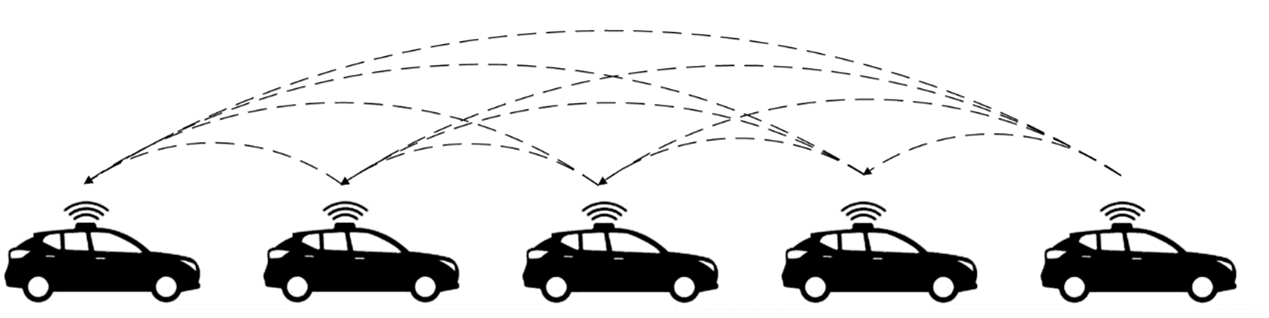
\includegraphics[width=14cm]{figs/fig1.png}
  \caption{~The schematic of the CAV platoon.}
  \label{fig1}
\end{figure}

Consider a group of n AVs moving along a single lane and forming a CAV platoon. Fig.~\ref{fig1} shows the schematic of the CAV platoon, where the dashed line denotes that there is communication between the two CAVs. It is worth mentioning that each CAV communicates with arbitrarily other CAVs in the platoon for the sake of generalization in the schematic. Nevertheless, the communication digraph is different in practice, depending on the different IFTs adopted. Via intra-vehicle communication (e.g., C-V2X according to the meeting report from Federal Communications Commission \citep{VerizonNorth2020}), all vehicles share their state information (e.g., the absolute position, velocity, and acceleration) with other vehicles within the platoon according to the IFT. It is assumed that each CAV is equipped with i) an on-board radar responsible for collision detection via measuring the gap distance between any two consecutive vehicles, ii) a built-in GPS sensor for measuring the longitudinal position, iii) a wireless on-board unit for communicating potentially useful information with its proximal vehicles via the C-V2X communication, iv) an upper-level controller for calculating the desired longitudinal acceleration based on the parameters obtained, and v) a lower-level controller for determining the throttle and brake actuator inputs to track the desired acceleration. Such an assumption is reasonable as the sensing, communication, and actuation units requested above are available in modern CAVs, and thus do not require specific changes in the existing vehicle configuration. Note that the on-board radar only functions when communication is unavailable or malfunctioning since more accurate information can be obtained via communication in a more efficient manner.

\subsection{Vehicle longitudinal dynamic Modeling}
\label{Section 3.1}

Let $p_i\left(t\right)$, $v_i\left(t\right)={\dot{p}}_i\left(t\right)$, $a_i\left(t\right)={\ddot{p}}_i\left(t\right)$, and $\ {\dot{a}}_i\left(t\right)={\dddot{p}}_i\left(t\right)\ \in\mathbb{R}$ denote the longitudinal position, speed, acceleration, and jerk of vehicle $i$ at time $t$, respectively. A vehicle longitudinal dynamic model mainly consists of the engine, throttle and brake actuators, drive train, transmission, and torque converter. Under a variety of resistance forces, the longitudinal dynamics of vehicle $i$ can be modeled by the following force balance equation:
\begin{equation}
  m_ia_i(t)=f_i^e(t)-f_i^g(t)-f_i^w(t)-f_i^r(t)
  \label{eq2}
\end{equation}
where $m_i$ stands for the unknown mass of vehicle $i$; $f_i^e(t)$ is the desired engine force acting on vehicle $i$; $f_i^g(t)$, $\ f_i^w(t)$, and $f_i^r(t)$ denote the gravity component parallel to the road surface, air resistance force, and rolling resistance force, respectively.

However, Equation~(\ref{eq2}) is nonlinear, which brings difficulty to the design of its controller. Hence a feedback control in Appendix B is employed to transfer Equation~(\ref{eq2}) into the linear form:
\begin{equation}
  \tau_i\dot{a_i}\left(t\right)+a_i\left(t\right)=u_i(t)
  \label{eq3}
\end{equation}
where $u_i(t)$ denotes the control input of the lower-level controller, which can be interpreted as the desired acceleration of vehicle $i$, $\tau_i$ is the time constant representing the engine actuator delay.

Reformulate Equation~(\ref{eq3}), the state space equation can be represented as:
\begin{equation}
  {\dot x_i}\left( t \right) = A{x_i}\left( t \right) + B{u_i}\left( t \right)
  \label{eq4}
\end{equation}
with $A = \left[ {\begin{array}{*{20}{c}}
          0 & 1 & 0                          \\
          0 & 0 & 1                          \\
          0 & 0 & { - \frac{1}{{{\tau _i}}}}
        \end{array}} \right]$ and $B = \left[ {\begin{array}{*{20}{c}}
          0 \\
          0 \\
          {\frac{1}{{{\tau _i}}}}
        \end{array}} \right]$\\
where ${x_i}\left( t \right) = {\left[ {\begin{array}{*{20}{c}}
          {{p_i}\left( t \right)} & {{v_i}\left( t \right)} & {{a_i}\left( t \right)}
        \end{array}} \right]^T} \in {\mathbb{R}^3}$ denotes the state vector of vehicle $i$.

As for the reference leading dynamics, it can be described as \citep{Hengster-Movric2015}:
\begin{equation}
  {\dot x_1}\left( t \right) = A{x_1}\left( t \right)
  \label{eq6}
\end{equation}
where ${x_1}\left( t \right) = {\left[ {\begin{array}{*{20}{c}}
          {{p_1}\left( t \right)} & {{v_1}\left( t \right)} & {{a_1}\left( t \right)}
        \end{array}} \right]^T} \in {\mathbb{R}^3}$.

As for the control strategy, due to the presence of limited communication, the control input of the vehicle $i$ is determined by an appropriate decentralized coupling protocol of communication information:
\begin{equation}
  {u_i} = {u_i}\underbrace {\left( {{x_1}\left( {t - h} \right), \cdots ,{x_i}\left( {t - {\text{h}}} \right), \cdots ,{x_n}\left( {t - h} \right)} \right)}_n
  \label{eq7}
\end{equation}\\
where $h$ represents the communication delay within the transmission range which is assumed to be similar among different IFTs \citep{Zheng2015,Vukadinovic2018,Vu2020,Martin-Sacristan2020,Pirani2022}.

Here we assume that CAVs adopt the Constant Distance (CD) policy and Leader-based IFT in which CAVs maintain a desired distance from the reference leader. Then the cooperative leader tracking problem can be formulated as follows:
\begin{equation}
  \left\{ \begin{gathered}
    \mathop {\lim }\limits_{t \to \infty } \left\| {{p_i}(t) - {p_1}(t) - {d_{i1}}} \right\| = 0 \hfill \\
    \mathop {\lim }\limits_{t \to \infty } \left\| {{v_i}(t) - {v_1}(t)} \right\| = 0 \hfill \\
    \mathop {\lim }\limits_{t \to \infty } \left\| {{a_i}(t) - {a_1}(t)} \right\| = 0 \hfill \\
  \end{gathered}  \right.\forall i = 1, \ldots ,N
  \label{eq8}
\end{equation}
where $d_{i1}$ denotes the desired intra-vehicle distance of vehicle $i$ from the leading vehicle.

The consensus goal (\ref{eq8}) can be achieved using an appropriate distributed strategy. Therefore, the vehicle $i$ adjusts its dynamics through the following decentralized coupling protocol computed onboard as:
\begin{equation}
  {u_i} =  - \sum\limits_{j = 1}^n {{a_{ij}}{k_{ij}}^T{{\left[ {\begin{array}{*{20}{c}}
              {{p_i}\left( {t - {h}} \right) - {p_j}\left( {t - {h}} \right) - {d_{ij}}} & {{v_i}\left( {t - {h}} \right) - {v_j}\left( {t - {h}} \right)} & {{a_i}\left( {t - {h}} \right) - {a_j}\left( {t - {h}} \right)}
            \end{array}} \right]}^T}}
  \label{eq9}
\end{equation}
where
\begin{itemize}
  \item[]
    ${a_{ij}}$ denotes the weight of the edge $\left( {i,j} \right)$, and ${a_{ij}} = 0$ if there is no edge $\left( {i,j} \right)$;                     \\
    ${d_{ij}}$ stands for the desired intra-vehicle distance of vehicle $i$ from the vehicle $j$;                                                        \\
    ${k_{ij}} = {\left[ {\begin{array}{*{20}{c}}
              {{\alpha _{ij}}} & {{\beta _{ij}}} & {{\gamma _{ij}}}
            \end{array}} \right]^T} \in {\mathbb{R}^{3}}$ presents the feedback control gain vector;                         \\
    ${\alpha _{ij}}$, ${\beta _{ij}}$, and ${\gamma _{ij}}$ denote the control gain of spacing error, speed error, and acceleration error, respectively.
\end{itemize}




\subsection{Closed-loop Vehicle Network Modeling}
\label{Section 3.2}

To prove the consensus of systems (\ref{eq4}) and (\ref{eq6}) under the action of coupling protocol (\ref{eq9}), we define the error state with respect to the leader as:
\begin{equation}
  {e_i}\left( t \right) = \left[ {\begin{array}{*{20}{c}}
          {{{\tilde p}_i}} \\
          {{{\tilde v}_i}} \\
          {{{\tilde a}_i}}
        \end{array}} \right] = \left[ {\begin{array}{*{20}{c}}
          {{p_i} - {p_1} - {d_{i1}}} \\
          {{v_i} - {v_1}}            \\
          {{a_i} - {a_1}}
        \end{array}} \right]
  \label{eq10}
\end{equation}

Then the decentralized coupling protocol (\ref{eq9}) can be reformulated as:
\begin{equation}
  {u_i} =  - \sum\limits_{j = 1}^n {{a_{ij}}{k_{ij}}^T\left[ {{e_i}(t - h) - {e_j}(t - h)} \right]}
  \label{eq11}
\end{equation}

Therefore, the dynamics of the error system can be presented as:
\begin{equation}
  \left\{ \begin{gathered}
    {{\dot {\tilde p}}_i} = {{\tilde v}_i} \hfill \\
    {{\dot {\tilde v}}_i} = {{\tilde a}_i} \hfill \\
    {{\dot {\tilde a}}_i} =  - \frac{1}{\tau }{{\tilde a}_i} - \frac{1}{\tau }\sum\limits_{j = 0}^n {{a_{ij}}{k_{ij}}^T\left( {{e_i}\left( {t - h} \right) - {e_j}\left( {t - h} \right)} \right)}  \hfill \\
  \end{gathered}  \right.
  \label{eq12}
\end{equation}

From Equation~(\ref{eq12}), the dynamics of the closed-loop vehicular network can be recast in a compact form as:
\begin{equation}
  {\dot e_i}\left( t \right) = A{e_i}\left( t \right) - B\sum\limits_{j = 0}^n {{a_{ij}}{k_{ij}}^T\left( {{e_i}\left( {t - h} \right) - {e_j}\left( {t - h} \right)} \right)}
  \label{eq13}
\end{equation}

\begin{theorem}
  \label{theo8}
  The closed-loop network system adopting constant communication delay, Leader-based IFT, and CD policy can be presented as a linear state delay system:
  \begin{equation}
    \left\{ \begin{gathered}
      \dot X\left( t \right) = {A^*}X\left( t \right) + \Psi X(t - h),\quad \forall t \geqslant 0 \hfill \\
      X\left( t \right) = \phi \left( t \right),\quad \quad \quad \quad \quad \quad \quad \forall t \in \left[ { - h,0} \right] \hfill \\
    \end{gathered}  \right.
    \label{eq14}
  \end{equation}
  with \\
  $\quad \left\{ {\begin{array}{*{20}{l}}
          {{A^*} = {I_n} \otimes A \in {\mathbb{R}^{3n \times 3n}}}                                                       \\
          {\Psi  =  - {B^*}\mathcal{F}\left( {{E_1} - {E_2}} \right) \in {\mathbb{R}^{3n \times 3n}}}                     \\
          {{B^*} = {I_n} \otimes B \in {\mathbb{R}^{3n \times n}}}                                                        \\
          \begin{gathered}
            \mathcal{K} = {[{k_{ij}}^T]_{n \times n}} \hfill \\
            \mathcal{H} = \mathcal{A}^\circ \mathcal{K} = {[{a_{ij}} \otimes {k_{ij}}^T]_{N \times N}} \in {\mathbb{R}^{n \times 3n}} \hfill \\
            \mathcal{F} = diag\underbrace {\left\{ {{\mathcal{H}_1},{\mathcal{H}_2}, \cdots ,{\mathcal{H}_N}} \right\}}_n \in {\mathbb{R}^{n \times 3{n^2}}} \hfill \\
            {\mathcal{H}_i} = \underbrace {\left[ {{a_{i1}}{k_{i1}}^T,{a_{i2}}{k_{i2}}^T, \cdots ,{a_{in}}{k_{in}}^T} \right]}_n \in {\mathbb{R}^{1 \times 3n}}\forall i \in \mathcal{V} \hfill \\
          \end{gathered}                                                                                      \\
          {{E_1} = diag\underbrace {\left\{ {{I_1},{I_1}, \cdots ,{I_1}} \right\}}_n \in {\mathbb{R}^{3{n^2} \times 3n}}} \\
          {{E_2} = {{\underbrace {\left[ {\begin{array}{*{20}{c}}
                            {{I_2}^T} & \cdots & {{I_2}^T}
                          \end{array}} \right]}_n}^T} \in {\mathbb{R}^{3{n^2} \times 3n}}} \\
          {{I_1} = {{\underbrace {\left[ {\begin{array}{*{20}{c}}
                            {{I_3}^T} & \cdots & {{I_3}^T}
                          \end{array}} \right]}_n}^T} \in {\mathbb{R}^{3n \times 3}}}      \\
          {{I_2} = {I_{3n}} \in {\mathbb{R}^{3n \times 3n}}}                                                              \\
          {{I_3} = {I_3} \in {\mathbb{R}^{3 \times 3}}}
        \end{array}} \right.$\\
  where $X\left( t \right) = {\left[ {\begin{array}{*{20}{c}}
            {{e_1}^T} & \cdots & {{e_n}^T}
          \end{array}} \right]^T} \in {\mathbb{R}^{3n}}$ stands for the error state vector of the closed-loop vehicular network; $\phi $ is the initial conditions; ${A^*}$ and $\Psi $ are constant matrix according to their definitions.

\end{theorem}
\begin{proof}
  \textbf{Theorem~\ref{theo8}} can be obtained by manipulating matrix transformations on the error state vector of the closed-loop vehicular network and Equation~(\ref{eq13}).
\end{proof}




\section{Stability analyses}
\label{Section 4}

The primary idea of Lemma~\ref{lemma1} is to determine a positive definite functional whose derivative with respect to time along the trajectories of the system (\ref{eq14}) is negative definite. Therefore, the local stability of the closed-loop network system (\ref{eq14}) can be guaranteed by proposing a candidate LKF $V$ and providing some conditions that guarantee its positive definiteness and the negative definiteness of its derivative. In the stability analysis of such systems using LKF, several types of functionals have been provided in the literature. Among them, an integral quadratic term is one of the most relevant components \citep{Fridman2003}:
\begin{equation}
  V\left( {{X_t}} \right) = \int_{ - h}^0 {\int_u^0 {\dot X_t^T} } (\theta )R{\dot X_t}(\theta ){\text{d}}\theta {\text{d}}u
  \label{eq16}
\end{equation}

Differentiating Equation~(\ref{eq16}) with respect to $t$ leads to:
\begin{equation}
  \dot V\left( {{X_t}} \right) = h\dot X_t^T(t)R{\dot X_t}(t) - \int_{ - h}^0 {\dot X_t^T} (u)R{\dot X_t}(u){\text{d}}u
  \label{eq17}
\end{equation}

In order to transform Equation~(\ref{eq17}) into a suitable LMI setup, an over-approximate process of the integral terms is adopted since it cannot be straightforwardly converted in the quadratic formulation described above.

Thanks to Lemma~\ref{lemma5}, the lower bound of $\int_{ - h}^0 {\dot X_t^T} (u)R{\dot X_t}(u){\text{d}}u$ can be derived by the following Corollary:
\begin{corollary}
  \label{corollary9}
  Let $x$ be such that $\dot x \in \mathcal{C}$, $R \in \mathbb{S}_n^ + $, and $h > 0$. Then, the integral inequality
  \begin{equation}
    \int_{ - h}^0 {{{\dot x}^T}} (u)R\dot x(u){\text{d}}u \geqslant \frac{1}{h}\xi _N^T\left[ {\sum\limits_{k = 0}^N {(2k + 1)} {\Gamma _N}{{(k)}^T}R{\Gamma _N}(k)} \right]{\xi _N},
    \label{eq18}
  \end{equation}
  holds for all integers $N \in \mathbb{N}$ where
  \begin{equation}
    {\xi _N} = \left\{ \begin{gathered}
      {\left[ {\begin{array}{*{20}{c}}
                {{x^T}(0)} & {{x^T}( - h)}
              \end{array}} \right]^T},\quad \quad \quad \quad \quad \quad \quad \quad \quad if\quad N = 0, \hfill \\
      {\left[ {\begin{array}{*{20}{c}}
              {{x^T}(0)} & {{x^T}( - h)} & {\frac{1}{h}\Omega _0^T} & \cdots & {\frac{1}{h}\Omega _{N - 1}^T}
            \end{array}} \right]^T},if\quad N > 0, \hfill \\
    \end{gathered}  \right.
    \label{eq19}
  \end{equation}
\end{corollary}
\begin{proof}
  See Appendix C for detailed proof.
\end{proof}

Define the lower bound by Corollary~\ref{corollary9}, and the stability theorem with an arbitrary $N$ follows.

\begin{theorem}
  \label{theorem10}
  For a given integer $N$ and a constant delay $h$, assume that there exists a matrix ${P_N} \in \mathbb{S}{_{\left( {N + 1} \right)n}}$ and two matrices $S,R \in \mathbb{S}_n^ + $ such that the LMIs
  \begin{equation}
    \label{lmi22}
    \begin{gathered}
      {\Theta _N}(h) = \left\{ {\begin{array}{*{20}{l}}
            {{P_N} \succ 0,}                                                                        & {{\text{ if }}N = 0} \\
            {{P_N} + \frac{1}{h}\operatorname{diag} \left( {{0_{nn}},{S_{N - 1}}} \right) \succ 0,} & {{\text{ if }}N > 0}
          \end{array}} \right. \hfill \\
      {\Phi _N}(h) = {\Phi _{N0}}(h) - {\left[ {\begin{array}{*{20}{c}}
              {{\Gamma _N}(0)} \\
              \vdots           \\
              {{\Gamma _N}(N)}
            \end{array}} \right]^T}{R_N}\left[ {\begin{array}{*{20}{c}}
              {{\Gamma _N}(0)} \\
              \vdots           \\
              {{\Gamma _N}(N)}
            \end{array}} \right] \prec 0 \hfill \\
    \end{gathered}
  \end{equation}
  hold, where \\
  \begin{equation}
    \left\{ \begin{gathered}
      {\Phi _{N0}}(h) = \operatorname{He} \left( {G_N^T(h){P_N}{H_N}} \right) + {{\tilde S}_N} + {h^2}F_N^TR{F_N}, \hfill \\
      {{\tilde S}_N} = \operatorname{diag} \left\{ {S, - S,{0_{Nn}}} \right\}, \hfill \\
      {S_N} = \operatorname{diag} \{ S,3S, \ldots ,(2N + 1)S\} , \hfill \\
      {F_N} = \left[ {\begin{array}{*{20}{l}}
              {{A^*}} & \Psi & {{0_{n,nN}}}
            \end{array}} \right], \hfill \\
      {G_N}(h) = \left[ {\begin{array}{*{20}{c}}
              I            & {{0_n}}      & {{0_{n,nN}}} \\
              {{0_{nN,n}}} & {{0_{nN,n}}} & {h{I_{nN}}}
            \end{array}} \right], \hfill \\
      {H_N} = {\left[ {\begin{array}{*{20}{l}}
                  {F_N^T} & {\Gamma _N^T(0)} & {\Gamma _N^T(1) \ldots \Gamma _N^T(N - 1)}
                \end{array}} \right]^T}. \hfill \\
    \end{gathered}  \right.
  \end{equation}
  Then system (\ref{eq14}) is asymptotically stable for the constant delay $h$.
\end{theorem}
\begin{proof}
  See Appendix D for detailed proof.
\end{proof}

\begin{remark}
  Taking $N=0$ in Theorem~\ref{theorem10} allows retrieving one of the most classical delay-dependent stability conditions based on Jensen's inequality and LMI \citep{Gouaisbaut2006}. Additionally, choosing $N=1$ leads to the stability conditions from \citet{Seuret2013}.
\end{remark}




\section{Numerical analyses}
\label{Section 5}

\subsection{Network and traffic scenario}
\label{Section 5.1}

\subsubsection{Simulation setting}
\label{Section 5.1.1}
To validate the theoretical results, we refer to a platoon consisting of five CAVs (as depicted in Fig.~\ref{fig1}) on a single-lane highway as a representative example. According to the definition of Leader-based IFTs, the leader communicates with all vehicles by broadcasting its information while other vehicles only communicate with their neighbors according to the IFT adopted. Here, we take the four most widely adopted Leader-based IFTs (Leader-Follower (LF), Leader-Predecessor-Follower (LPF), Leader-Multiple-predecessors-Follower (LMPF), and Leader-Bi-Direction (LBD)) as an example to analyze tracking performance and safety. The caveat is that although parameters should be selected based on the specific control structure in practical. In order to obtain a simulation result for further analysis, the parameters for both network and traffic simulation are reported in Table~\ref{table1} for simplicity but without loss of generality. Note that the weighted adjacent matrix is set to ${a_{ij}} = \frac{1}{{{d_i}}},\forall (i,j) \in \mathcal{E}$ denote that all the information of neighbors is playing an equal role in control decisions. Moreover, different CAV set different control gains to simulate heterogeneity.

\begin{table}
  \centering

  \setlength{\abovecaptionskip}{0pt}
  \setlength{\belowcaptionskip}{10pt}%设置标题与表格的距离
  \begin{threeparttable}[b]
    \caption{~Network and traffic simulation parameters.}
    {\begin{tabular}{lc} \toprule
        Parameters                                         & Value                                         \\ \midrule
        Platoon size $n$                                   & 5 vehicles                                    \\
        Vehicle length $L$                                 & 5 [m]                                         \\
        Engine actuator delay $\tau_i$                     & 0.2 [s] \tnote{1}                             \\
        Communication delay $h$                            & 0.3 [s] \tnote{2}                             \\
        Weight of edge $\left( {i,j} \right) \quad a_{ij}$ & $\frac{1}{{{d_i}}}$                           \\
        Feedback control gain vector $k_{ij}$              & $\left\{ \begin{gathered}
            {[0.2,0.4,0.2]^T}\quad for \quad i = 2; \hfill \\
            {[0.3,0.3,0.2]^T}\quad for \quad i = 3; \hfill \\
            {[0.3,0.4,0.3]^T}\quad for \quad i = 4; \hfill \\
            {[0.3,0.4,0.2]^T}\quad for \quad i = 5. \hfill \\
          \end{gathered}  \right.$ \\
        Desired intra-vehicle distance $d_{ij}$            & 15 [m]                                        \\
        \bottomrule
        \label{table1}
      \end{tabular}}
    \begin{tablenotes}
      \item[1] \citep{Wang2018a,Zhou2020}
      \item[2] \citep{Abbas2018,Thota2019}
    \end{tablenotes}
  \end{threeparttable}
\end{table}

\subsubsection{Introduction to the common Leader-based IFTs}
\label{Section 5.1.2}

\begin{figure}
  \centering
  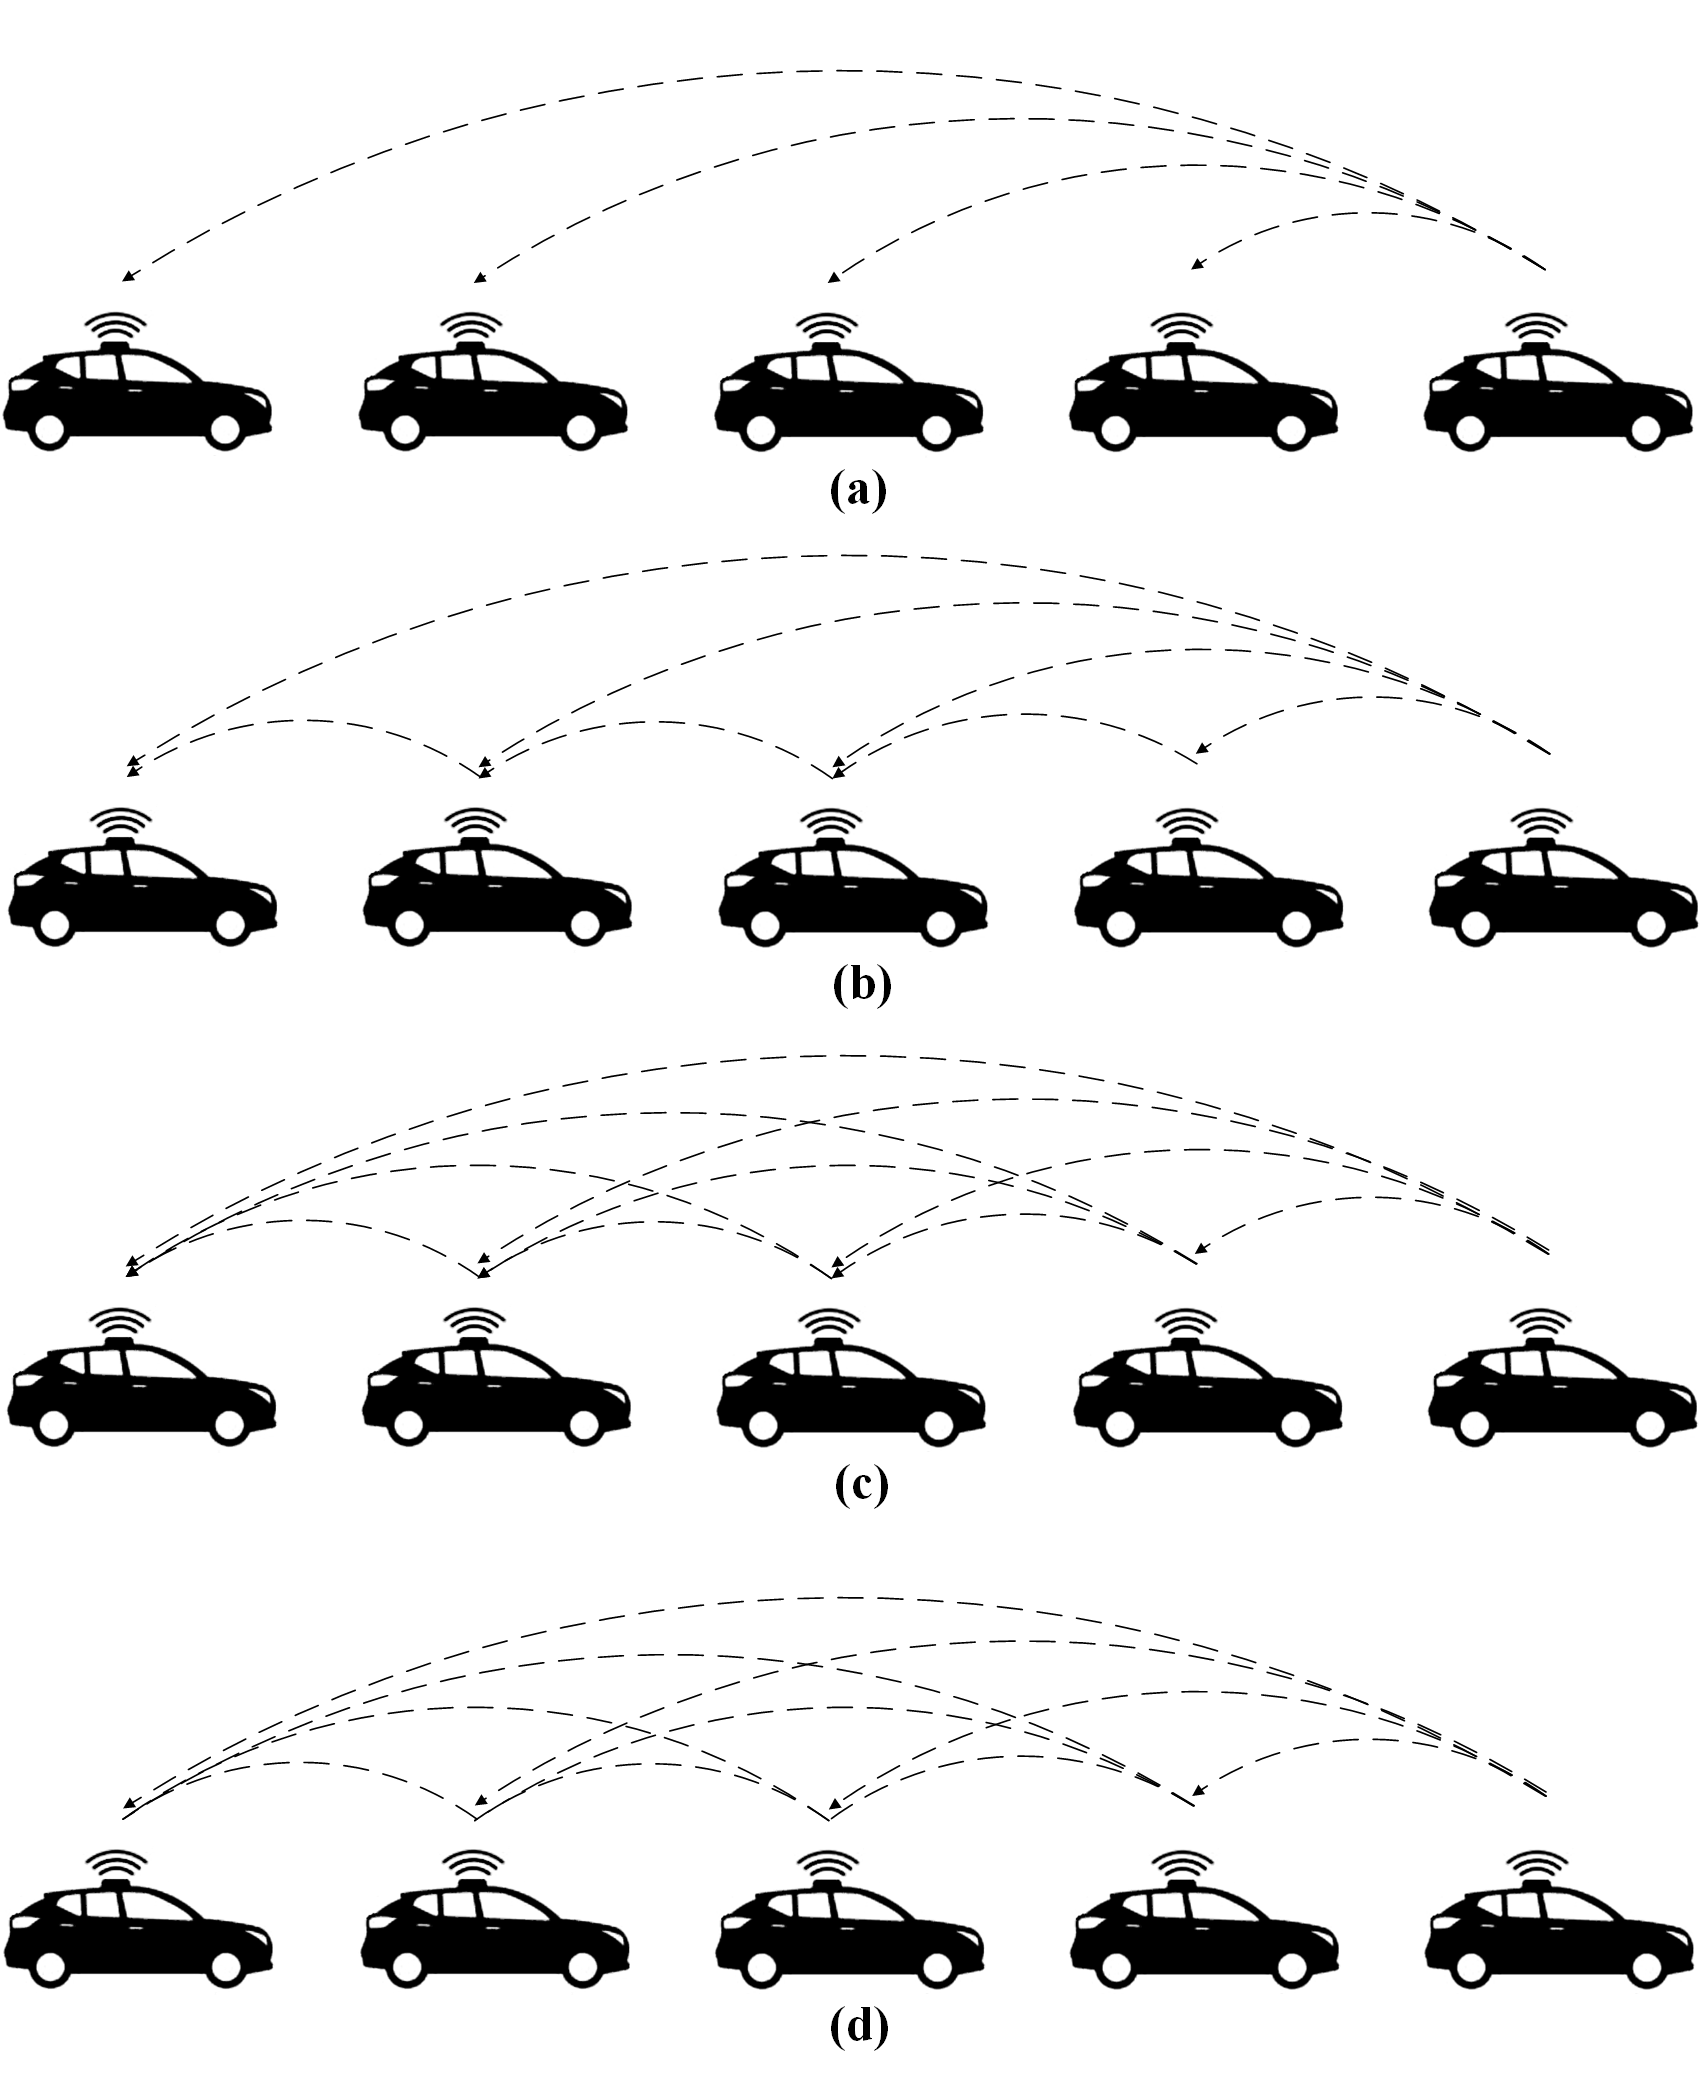
\includegraphics[width=12cm]{figs/fig2.png}
  \caption{~The communication schematic of typical three Leader-based IFTs for the CAV platoon: (a) Leader-Follower (LF); (b) Leader-Predecessor-Follower (LPF); (c) Leader-Multiple-predecessors-Follower (LMPF); and (d) Leader-Bi-Direction (LBD), where dotted lines with an arrow denote the one-direction communication while dotted lines without arrows represent the bi-direction communication.}
  \label{fig2}
\end{figure}

In this section, we give a detailed introduction to the four most widely adopted Leaders-based IFTs (LF, LPF, LMPF, and LBD) and the corresponding derivation of the dynamic equation. The communication schematic of the typical four Leader-based IFTs is shown in Fig.~\ref{fig2}, where dotted lines with an arrow denote the one-direction communication while dotted lines without arrows represent the bi-direction communication.


\textbf{\emph{The case of LF}}

For LF, all CAVs in the platoon only obtain information from the leader. The Equation (\ref{eq11}) can be reformed as follows:
\begin{equation}
  {u_i}(t) = {a_{i1}}{k_{i1}}^T\left[ {{e_i}(t - h) - {e_1}(t - h)} \right]
  \label{eq51}
\end{equation}

Substitute Equation (\ref{eq51}) into Equation (\ref{eq3}), the dynamic equation of LF can be obtained as:
\begin{equation}
  \begin{gathered}
    {{\dot a}_i}\left( t \right) =  - \frac{1}{{{\tau _i}}}{a_{i1}}\left[ {{\alpha _{i1}}({{\tilde p}_i}(t - h) - {{\tilde p}_1}(t - h)) + {\beta _{i1}}({{\tilde v}_i}(t - h) - {{\tilde v}_1}(t - h)) + {\gamma _{i1}}({{\tilde a}_i}(t - h) - {{\tilde a}_1}(t - h))} \right] - \frac{1}{{{\tau _i}}}{a_i}\left( t \right) \hfill \\
    \quad \quad  =  - \frac{1}{{{\tau _i}}}{a_{i1}}\left[ {{\alpha _{i1}}{{\tilde p}_i}(t - h) + {\beta _{i1}}{{\tilde v}_i}(t - h) + {\gamma _{i1}}{{\tilde a}_i}(t - h)} \right] - \frac{1}{{{\tau _i}}}{a_i}\left( t \right) \hfill \\
    \quad \quad  =  - \frac{1}{{{\tau _i}}}{a_{i1}}\left[ {{\alpha _{i1}}\left( {{p_i}(t - h) - {p_1}(t - h) - {d_{i1}}} \right) + {\beta _{i1}}\left( {{v_i}(t - h) - {v_1}(t - h)} \right){\text{ + }}{\gamma _{i1}}\left( {{a_i}(t - h) \!-\! {a_1}(t - h)} \right)} \right] - \frac{1}{{{\tau _i}}}{a_i}\left( t \right) \hfill \\
  \end{gathered}
  \label{eq52}
\end{equation}

\textbf{\emph{The case of LPF}}

As for LPF, all CAVs in the platoon obtain information from both the leader and the immediate predecessor. The decentralized coupling protocol (\ref{eq11}) can be reformed as follows:
\begin{equation}
  {u_i} =  - {a_{i1}}{k_{i1}}^T\left[ {{e_i}(t - h) - {e_1}(t - h)} \right] - {a_{i(i - 1)}}{k_{i(i - 1)}}^T\left[ {{e_i}(t - h) - {e_{i - 1}}(t - h)} \right]
  \label{eq53}
\end{equation}

Then, the dynamic equation of LPF can be obtained as:
\begin{equation}
  \begin{gathered}
    {{\dot a}_i}\left( t \right) =  - \frac{1}{{{\tau _i}}}{a_i}\left( t \right) - \frac{1}{{{\tau _i}}}\left[ {{a_{i1}}\left[ {{\alpha _{i1}}({{\tilde p}_i}(t - h) - {{\tilde p}_1}(t - h)) + {\beta _{i1}}({{\tilde v}_i}(t - h) - {{\tilde v}_1}(t - h)) + {\gamma _{i1}}({{\tilde a}_i}(t - h) - {{\tilde a}_1}(t - h))} \right]} \right. \hfill \\
    \quad \quad \quad \quad \quad \quad \quad \quad \quad  + {a_{i(i - 1)}}\left[ {{\alpha _{i(i - 1)}}\left( {{{\tilde p}_i}(t - h) - {{\tilde p}_{i - 1}}(t - h)} \right) + {\beta _{i(i - 1)}}\left( {{{\tilde v}_i}(t - h) - {{\tilde v}_{i - 1}}(t - h))} \right)} \right. \hfill \\
    \quad \quad \quad \quad \quad \quad \quad \quad \quad \quad \quad \quad \quad {\kern 1pt} \left. {{\gamma _{i(i - 1)}}({{\tilde a}_i}(t - h) - {{\tilde a}_{i - 1}}(t - h))} \right] \hfill \\
    \quad \quad  =  - \frac{1}{{{\tau _i}}}{a_i}\left( t \right) - \frac{1}{{{\tau _i}}}\left[ {{a_{i1}}\left[ {{\alpha _{i1}}\left( {{p_i}(t - h) - {p_1}(t - h) - {d_{i1}}} \right) + {\beta _{i1}}\left( {{v_i}(t - h) - {v_1}(t - h)} \right){\text{ + }}{\gamma _{i1}}\left( {{a_i}(t - h) - {a_1}(t - h)} \right)} \right]} \right. \hfill \\
    \quad \quad \quad \quad \quad \quad \quad \quad \quad  + {a_{i(i - 1)}}\left[ {{\alpha _{i(i - 1)}}\left( {{p_i}(t - h) - {p_{i - 1}}(t - h) - {d_{i(i - 1)}}} \right) + {\beta _{i(i - 1)}}\left( {{v_i}(t - h) - {v_{i - 1}}(t - h)} \right)} \right. \hfill \\
    \quad \quad \quad \quad \quad \quad \quad \quad \quad \quad \quad \quad \quad {\kern 1pt} \left. {{\text{ + }}{\gamma _{i(i - 1)}}\left( {{a_i}(t - h) - {a_{i - 1}}(t - h)} \right)} \right] \hfill \\
  \end{gathered}
  \label{eq54}
\end{equation}

\textbf{\emph{The case of LMPF}}

In addition, for LMPF, all CAVs in the platoon are able to obtain information from the leader and all predecessors. The decentralized coupling protocol (\ref{eq11}) can be reformed as follow:
\begin{equation}
  {u_i} =  - \sum\limits_{j = 1}^{i - 1} {{a_{ij}}{k_{ij}}^T\left[ {{e_i}(t - h) - {e_j}(t - h)} \right]}
  \label{eq55}
\end{equation}

The dynamic equation of LMPF can be presented as:
\begin{equation}
  \begin{gathered}
    {{\dot a}_i}\left( t \right) =  - \frac{1}{{{\tau _i}}}{a_i}\left( t \right) \hfill \\
    \;\;\;{\kern 1pt} \;\;\;{\kern 1pt} \;\;\;{\kern 1pt}  - \frac{1}{{{\tau _i}}}\sum\limits_{j = 1}^{i - 1} {{a_{ij}}\left[ {{\alpha _{ij}}({{\tilde p}_i}(t - h) - {{\tilde p}_j}(t - h)) + {\beta _{ij}}({{\tilde v}_i}(t - h) - {{\tilde v}_j}(t - h)) + {\gamma _{ij}}({{\tilde a}_i}(t - h) - {{\tilde a}_j}(t - h))} \right]}  \hfill \\
    \quad \quad  =  - \frac{1}{{{\tau _i}}}{a_i}\left( t \right) \hfill \\
    \;\;\;{\kern 1pt} \;\;\;{\kern 1pt} \;\;\; - \frac{1}{{{\tau _i}}}\sum\limits_{j = 1}^{i - 1} {{a_{ij}}\left[ {{\alpha _{ij}}\left( {{p_i}(t - h) - {p_j}(t - h) - {d_{ij}}} \right) + {\beta _{ij}}\left( {{v_i}(t - h) - {v_j}(t - h)} \right){\text{ + }}{\gamma _{ij}}\left( {{a_i}(t - h) - {a_j}(t - h)} \right)} \right]}  \hfill \\
  \end{gathered}
  \label{eq56}
\end{equation}

\textbf{\emph{The case of LBD}}

For LBD, all CAVs in the platoon except the leader are able to obtain information from each vehicle. The decentralized coupling protocol can still be represented by Equation (\ref{eq11}). The dynamic equation of LBD can be presented as:
\begin{equation}
  \begin{gathered}
    {{\dot a}_i}\left( t \right) =  - \frac{1}{{{\tau _i}}}{a_i}\left( t \right) \hfill \\
    \;\;\;{\kern 1pt} \;\;\;{\kern 1pt} \;\;\;{\kern 1pt}  - \frac{1}{{{\tau _i}}}\sum\limits_{j = 1}^n {{a_{ij}}\left[ {{\alpha _{ij}}({{\tilde p}_i}(t - h) - {{\tilde p}_j}(t - h)) + {\beta _{ij}}({{\tilde v}_i}(t - h) - {{\tilde v}_j}(t - h)) + {\gamma _{ij}}({{\tilde a}_i}(t - h) - {{\tilde a}_j}(t - h))} \right]}  \hfill \\
    \quad \quad  =  - \frac{1}{{{\tau _i}}}{a_i}\left( t \right) \hfill \\
    \;\;\;{\kern 1pt} \;\;\;{\kern 1pt} \;\;\; - \frac{1}{{{\tau _i}}}\sum\limits_{j = 1}^n {{a_{ij}}\left[ {{\alpha _{ij}}\left( {{p_i}(t - h) - {p_j}(t - h) - {d_{ij}}} \right) + {\beta _{ij}}\left( {{v_i}(t - h) - {v_j}(t - h)} \right){\text{ + }}{\gamma _{ij}}\left( {{a_i}(t - h) - {a_j}(t - h)} \right)} \right]}  \hfill \\
  \end{gathered}
  \label{eq57}
\end{equation}

\subsection{Tracking performance of Leader-based IFTs}

Firstly, in the preliminary analysis, we start considering the tracking performance of the four IFTs studied. From this perspective, the tracking performances have been evaluated considering two representative leader maneuvers, namely:
\begin{enumerate}
  \item \textbf{Trapezoidal signal}: The leader suddenly decelerates to 14.6m/s at $-0.15m/s^2$ and keeps it for 36s. Then the leader accelerates back to 20m/s at   $0.3m/s^2$ (see Fig.~\ref{fig3}(a, b)).
  \item \textbf{Oscillation signal}: The leader suddenly accelerates to 23.6m/s in 12s and keeps the velocity for 15s. Then the leader decelerates to 16.4m/s in 12s and accelerates back to 20m/s in 12s (see Fig.~\ref{fig3}(c, d)).
\end{enumerate}

\begin{figure}
  \centering
  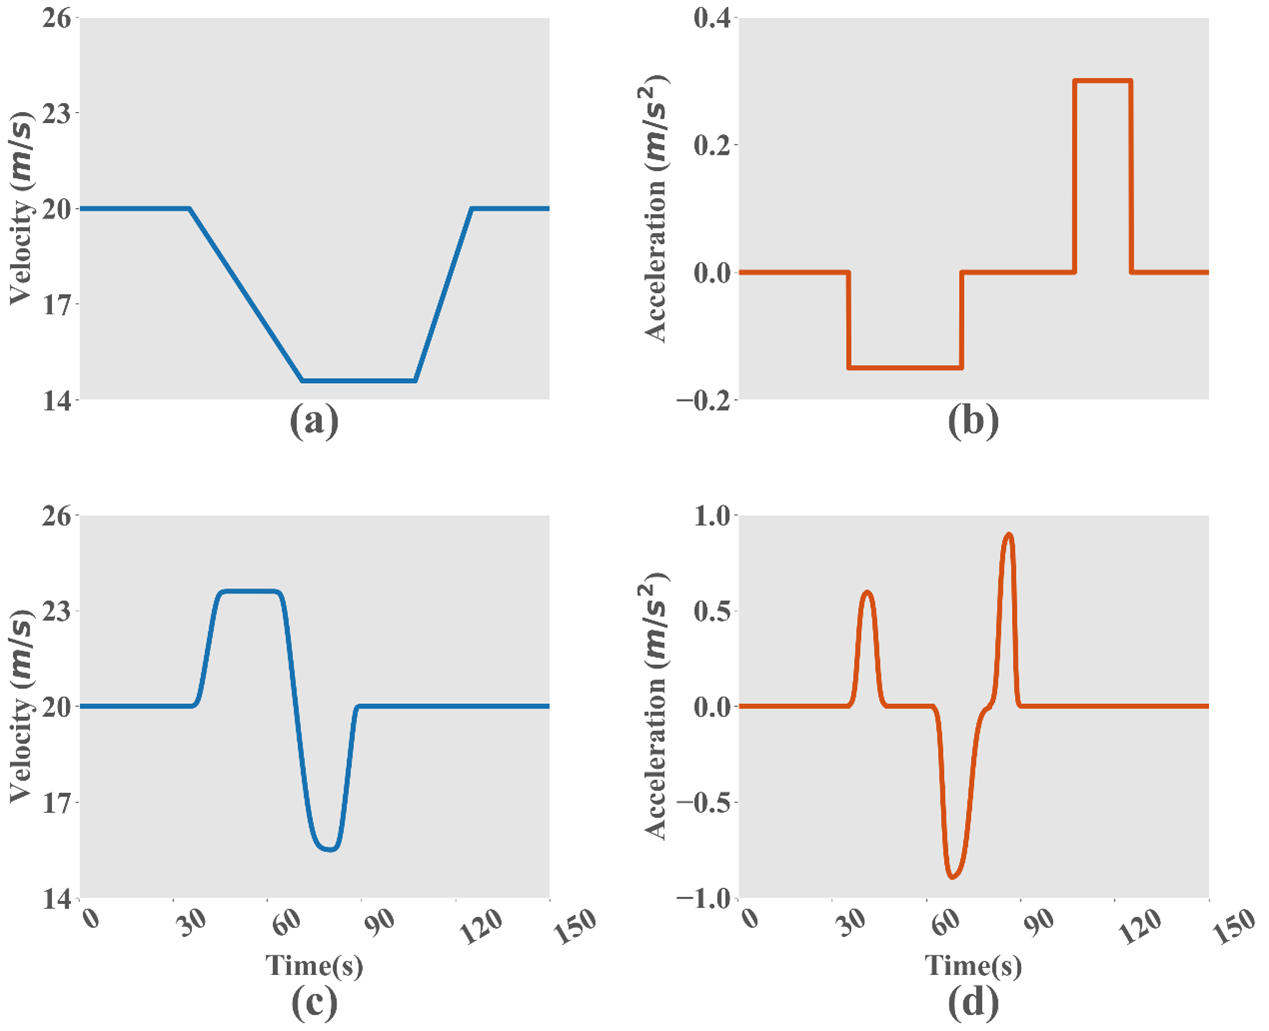
\includegraphics[width=14cm]{figs/fig3.png}
  \caption{~The two representative leader maneuvers: (a) and (b) denote the velocity and acceleration of the trapezoidal signal, respectively; (c) and (d) denote the velocity and acceleration of the oscillation signal, respectively.}
  \label{fig3}
\end{figure}

Once the platoon is formed and all CAVs reach the equilibrium state where the tracking error is 0, we adopt the trapezoidal signal in Fig.~\ref{fig3}(a, b) as the leader maneuver to test the tracking performance of the four IFTs. Results in Fig.~\ref{fig4} confirm the theoretical analysis and show how CAVs track the lead. As expected, all CAVs in the platoon enable fast and smooth tracking of the motion of the leader. Besides, transient changes in the reference signal arise abrupt changes in the tracking error. Nevertheless, such errors are diminished over time thanks to the stability property. In addition, the tracking speed and overshoot of different CAV amounts for transient responses to changes in the reference signal are different due to different control gains adopted.

\begin{figure}
  \centering
  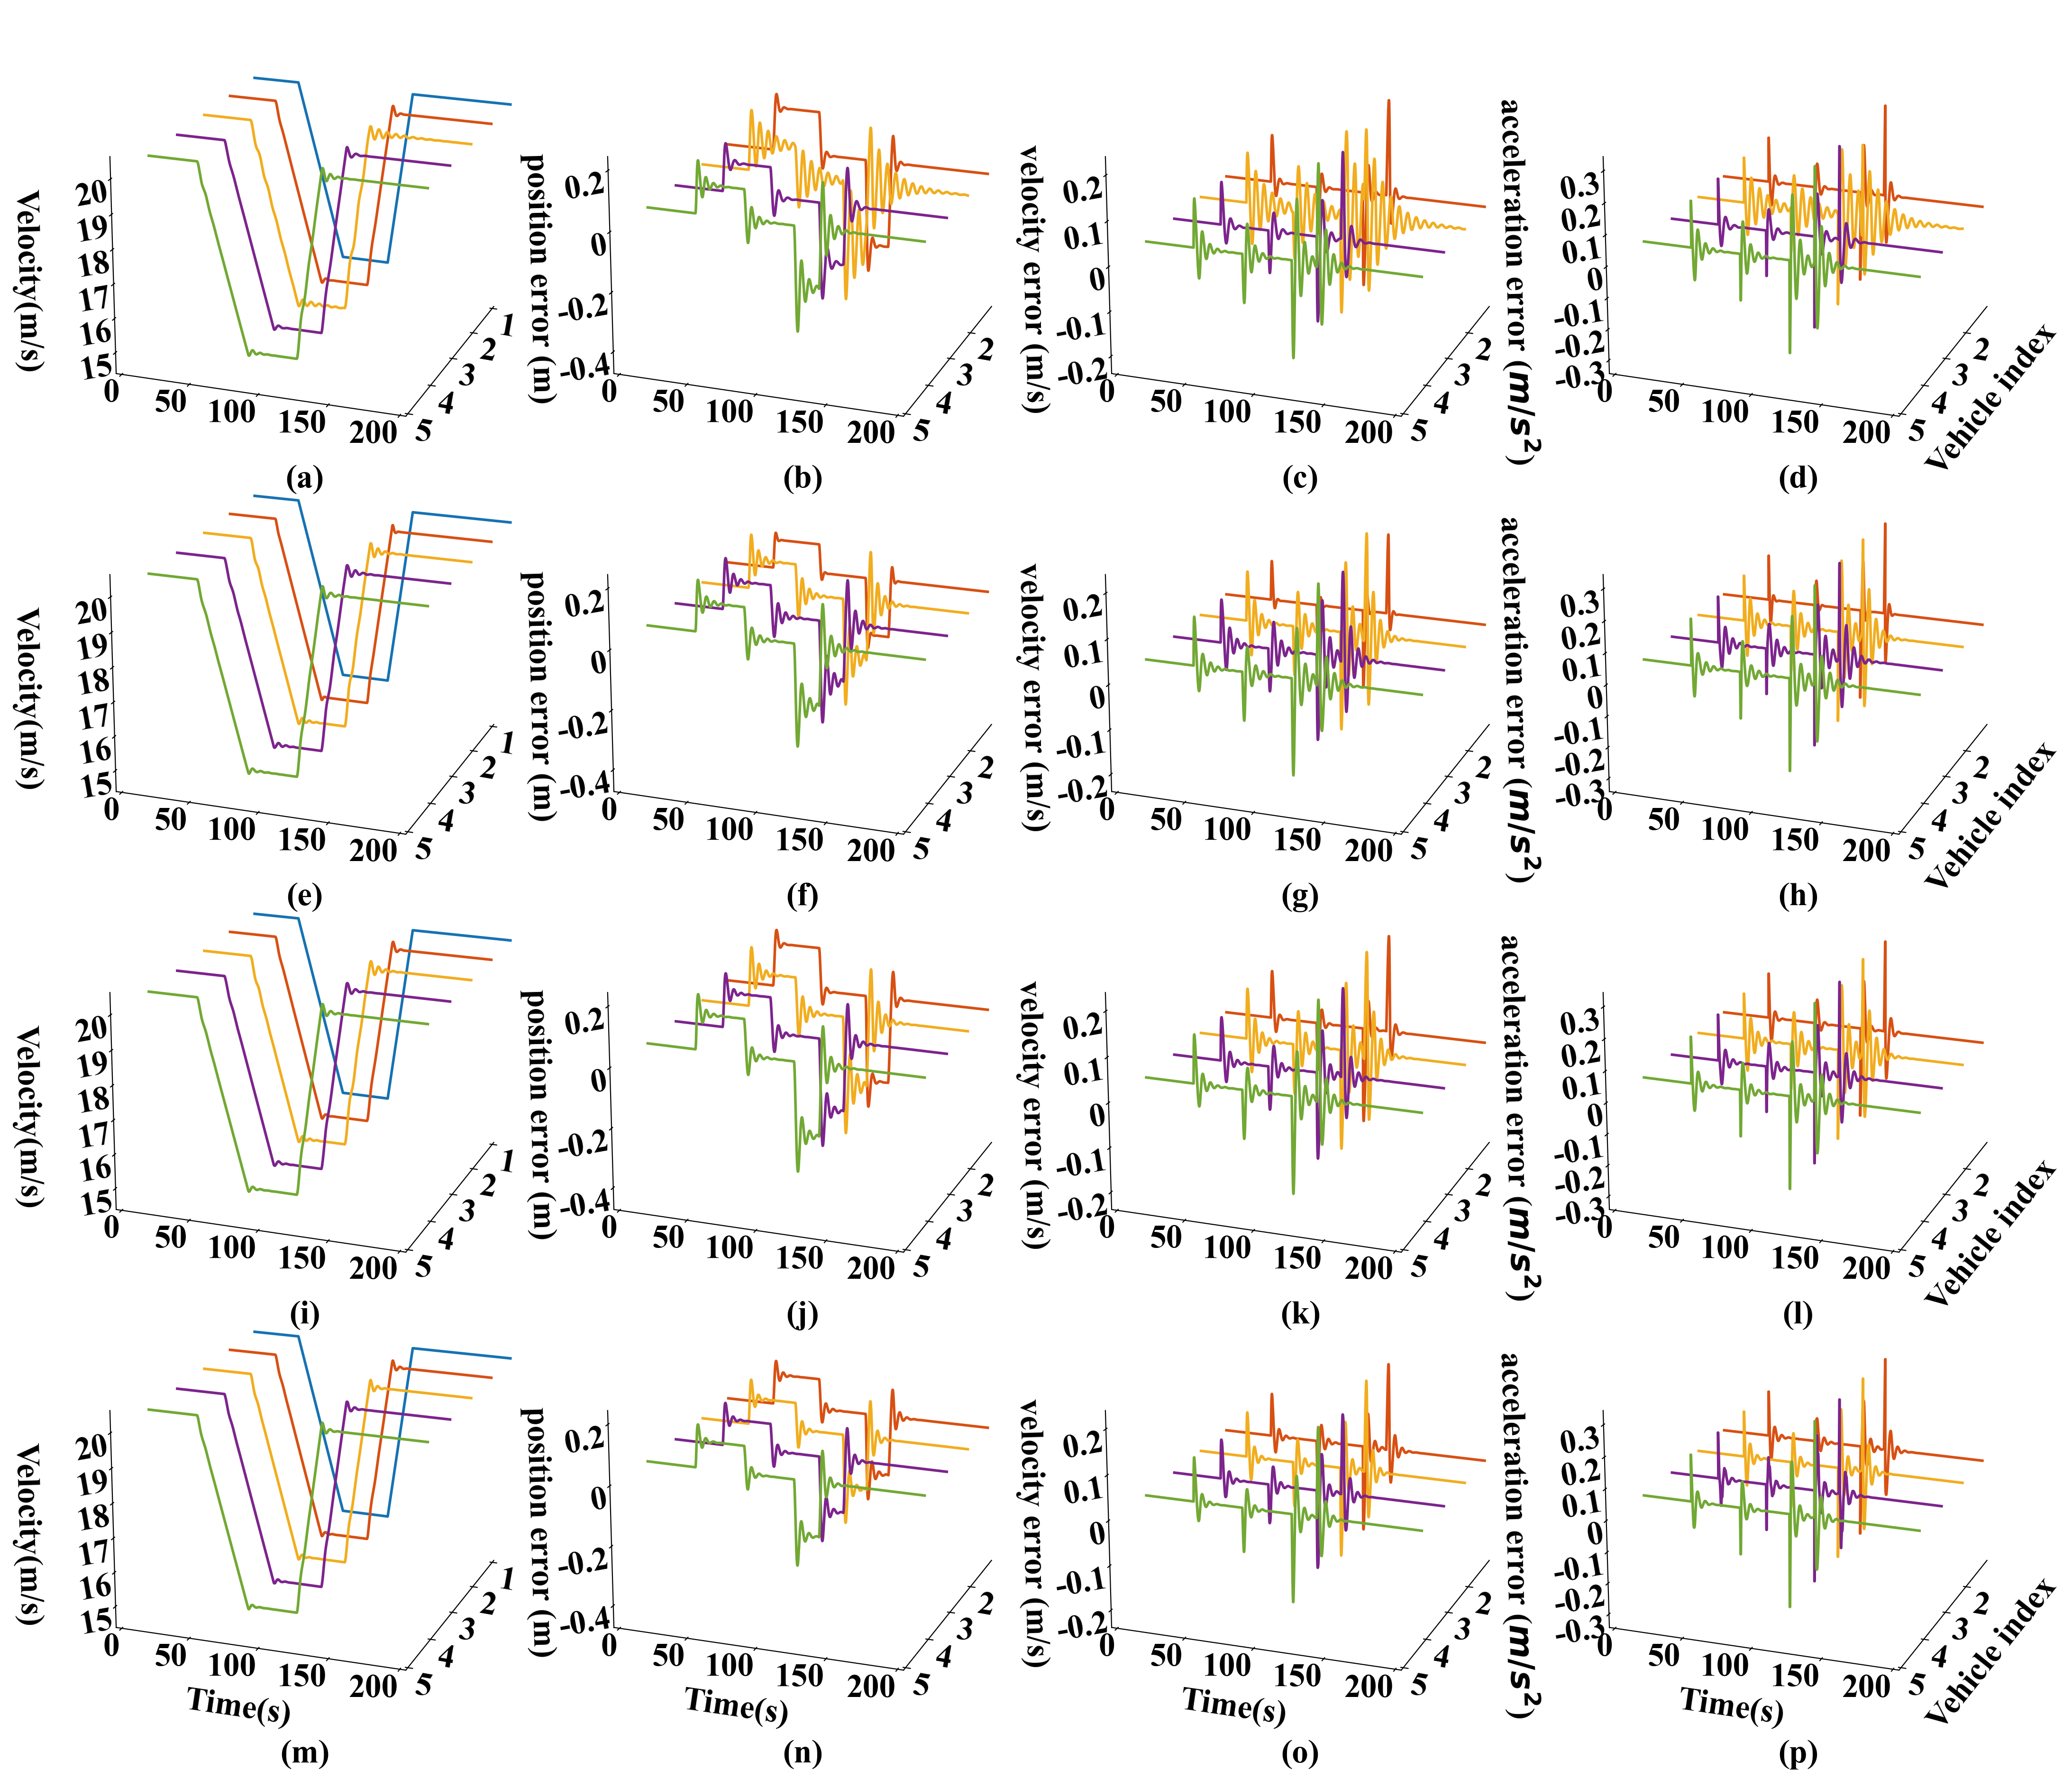
\includegraphics[width=14cm]{figs/fig4.png}
  \caption{~Tracking performance for the Trapezoidal signal in Fig. 3(a,b) under the four IFTs: (a), (b), (c), and (d) present tracking results under LF, including the velocity, tracking error of position, tracking error of velocity, and tracking error of acceleration, respectively; (e), (f), (g), and (h) show the case under LPF; (i), (j), (k), and (l) denote the case under LMPF; (m), (n), (o), and (p) show the case under LBD.}
  \label{fig4}
\end{figure}


Besides, the tracking performance of the four IFTs has also been tested here for the oscillation signal defined in Fig.~\ref{fig3}(c, d). In this case, Fig.~\ref{fig5} shows the tracking performance of the four IFTs. It demonstrates excellent cooperative tracking behavior since each CAV can track the reference signal steadily while maintaining the rigid formation requirements. Moreover, the tracking error is caused by transient changes in the reference signal and decays smoothly over time, as in the case of the trapezoidal signal. Furthermore, Figs.~\ref{fig4},\ref{fig5} verify the effectiveness of the four IFTs on tracking performance and stability.

\begin{figure}
  \centering
  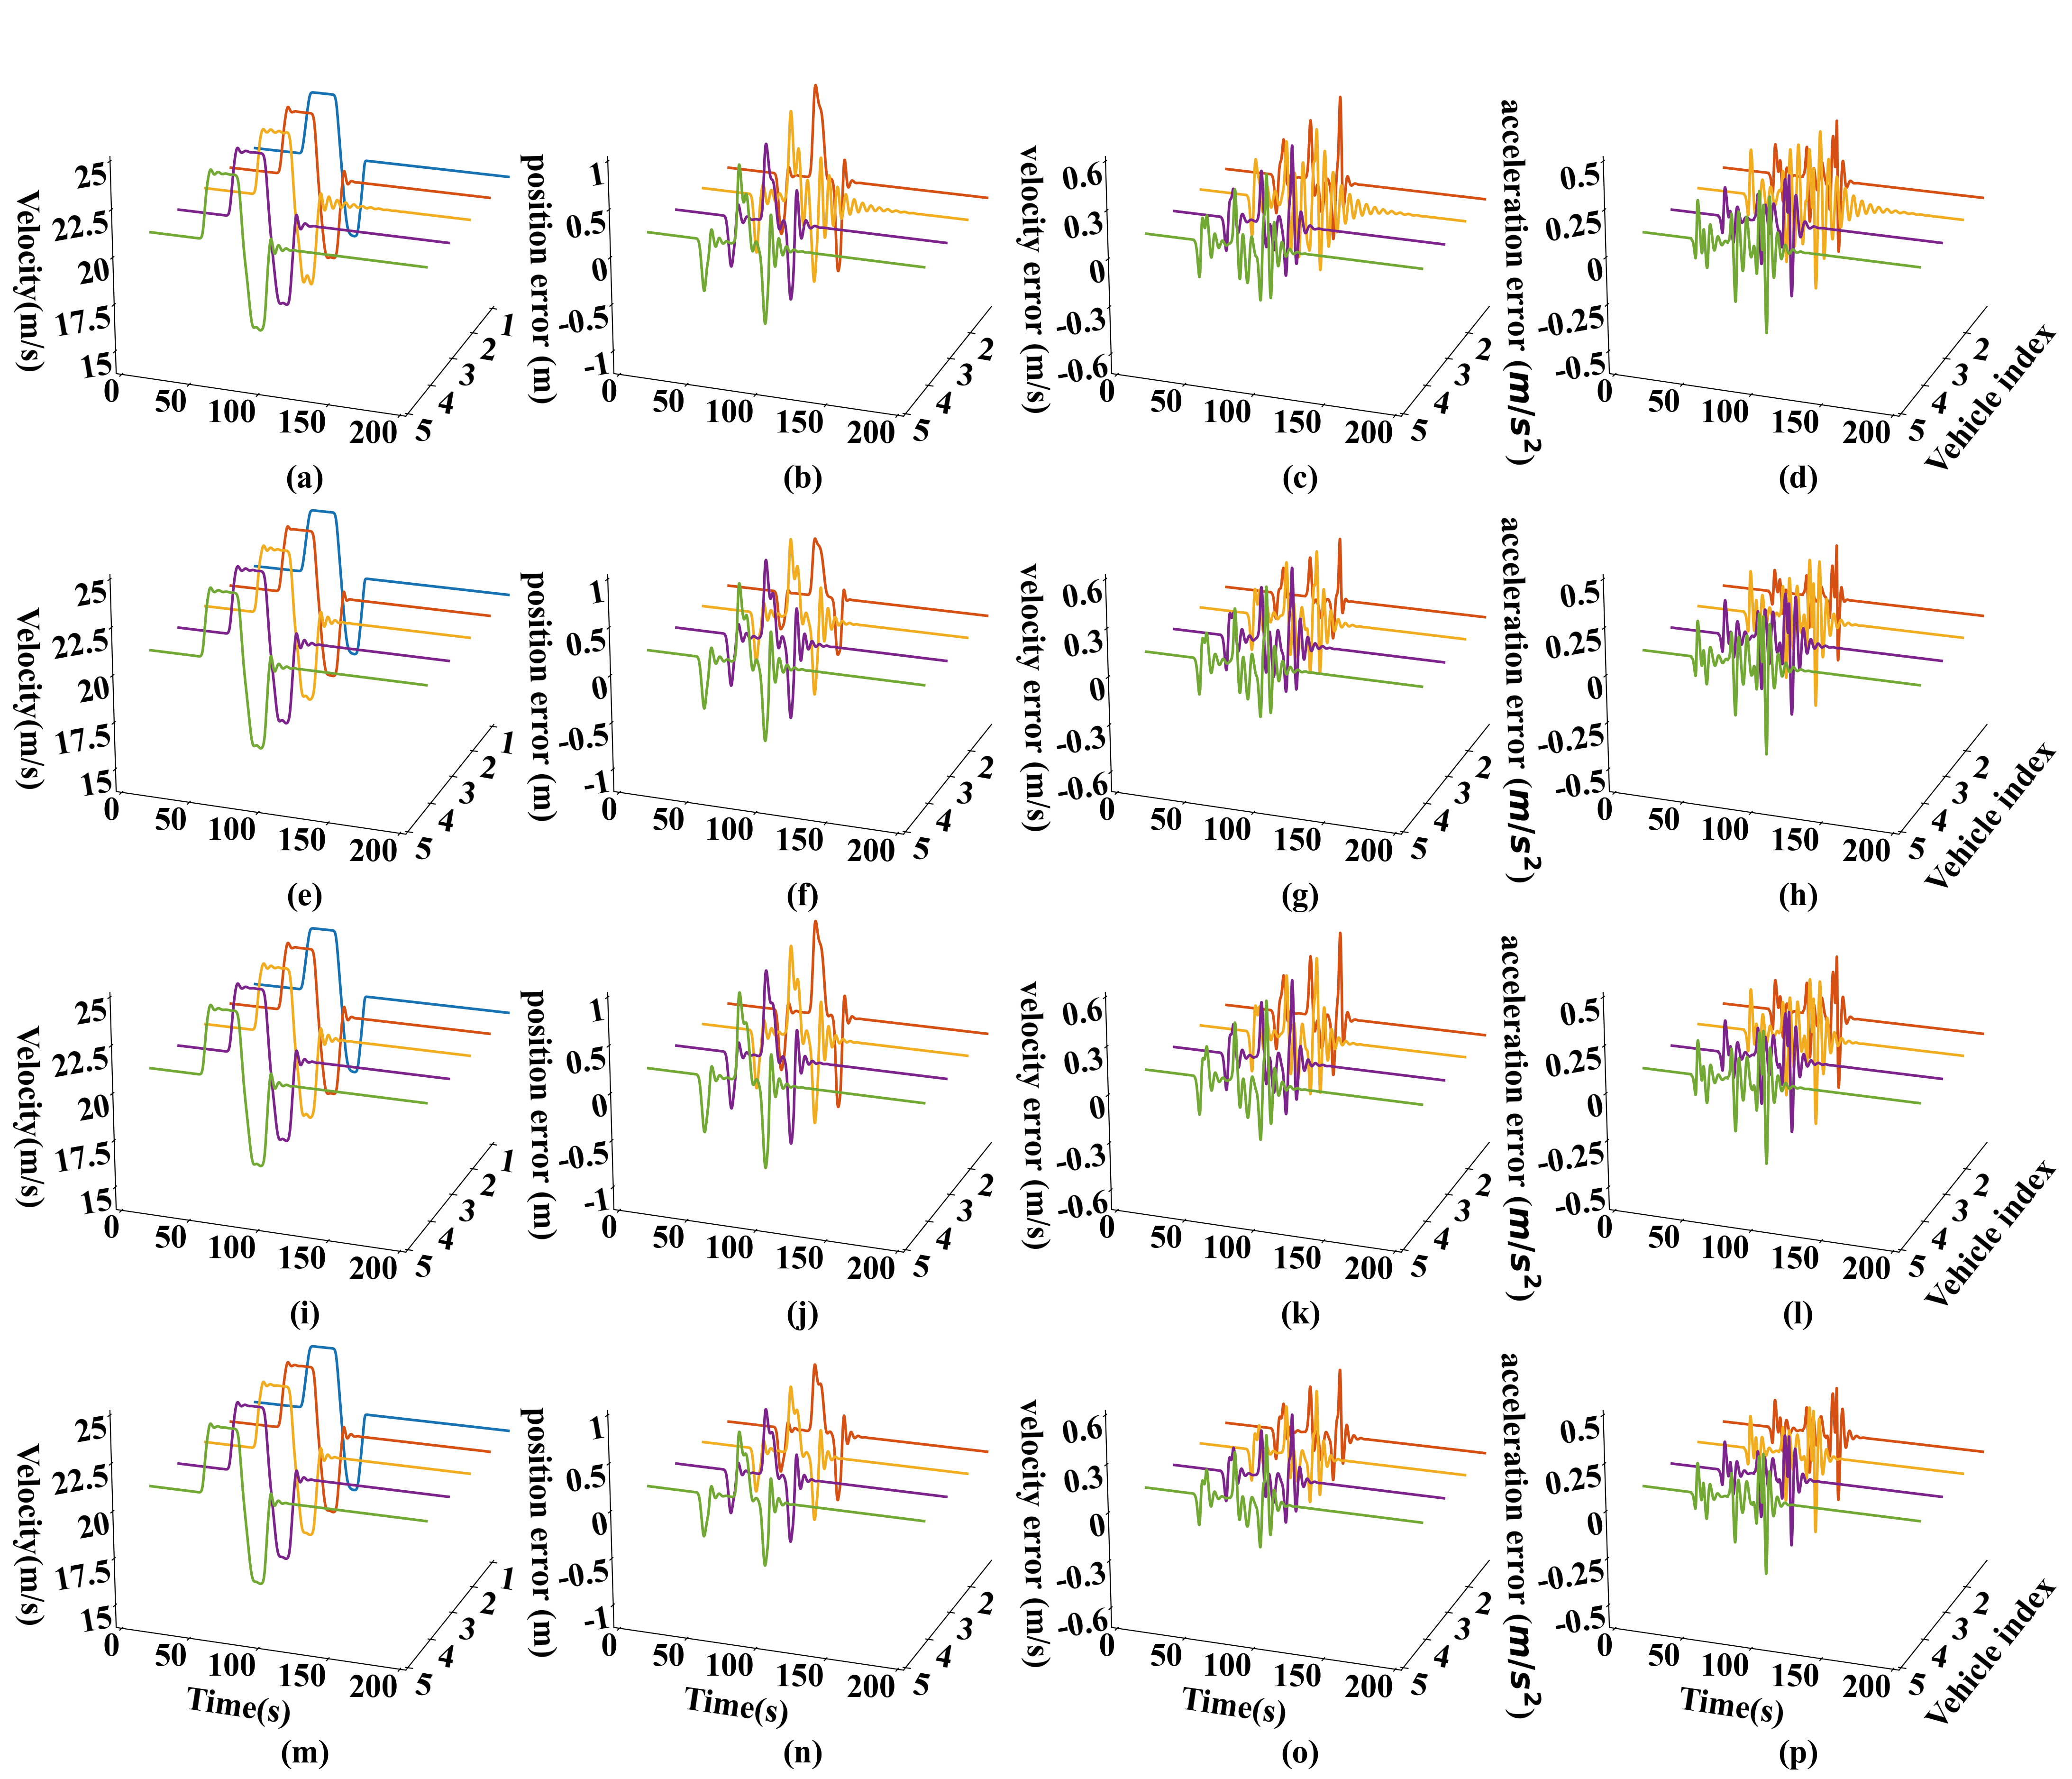
\includegraphics[width=14cm]{figs/fig5.png}
  \caption{~Tracking performance for the Oscillation signal in Fig. 3(c,d) under the four IFTs: (a), (b), (c), and (d) present tracking results under LF, including the velocity, tracking error of position, tracking error of velocity, and tracking error of acceleration, respectively; (e), (f), (g), and (h) show the case under LPF; (i), (j), (k), and (l) denote the case under LMPF; (m), (n), (o), and (p) show the case under LBD.}
  \label{fig5}
\end{figure}


\subsection{Safety analyses considering hard braking maneuver}

To further evaluate the safety in all the different driving and communication scenarios, we have also quantitatively analyzed the possible emergence of critical driving situations for all IFTs under investigation by exploiting the safety indicator Deceleration Rate to Avoid the Crash (DRAC), which is well known in the literature \citep{saccomanno2008comparing,fu2021comparison}. This indicator presents the deceleration rate needed to be applied by a vehicle to avoid a collision with another vehicle which can be defined for each vehicle $i$ at the time $t$ as follows:
\begin{equation}
  DRA{C_i}(t) = \frac{{{{\left( {{v_i}(t) - {v_{i - 1}}(t)} \right)}^2}}}{{2\left( {{p_{i - 1}}(t) - {p_i}(t) - L} \right)}}
  \label{eqsafe}
\end{equation}

Moreover, we consider here the occurrence of hard braking (emergency) maneuver as an additional evaluation scenario. Specifically, results in Fig.~\ref{fig6} show how the platoon reacts in the case of a braking maneuver performed by the leader for each IFT under investigation. Once again, in this case, all CAVs under each IFT smoothly track the motion of the leader during hard braking avoiding possible collisions. Furthermore, the variation of selected safety indicator DRAC over time under different IFTs is shown in Fig.~\ref{fig7} to explore the changes in the security situation under the hard braking maneuver. It is worth mentioning that the variation of the leader is omitted since it has no predecessor, which will raise the risk of collisions. Besides, the CAV2, CAV3, CAV4, and CAV5 refer to the second, third, fourth, and fifth CAV in the CAV platoon, respectively.

\begin{figure}
  \centering
  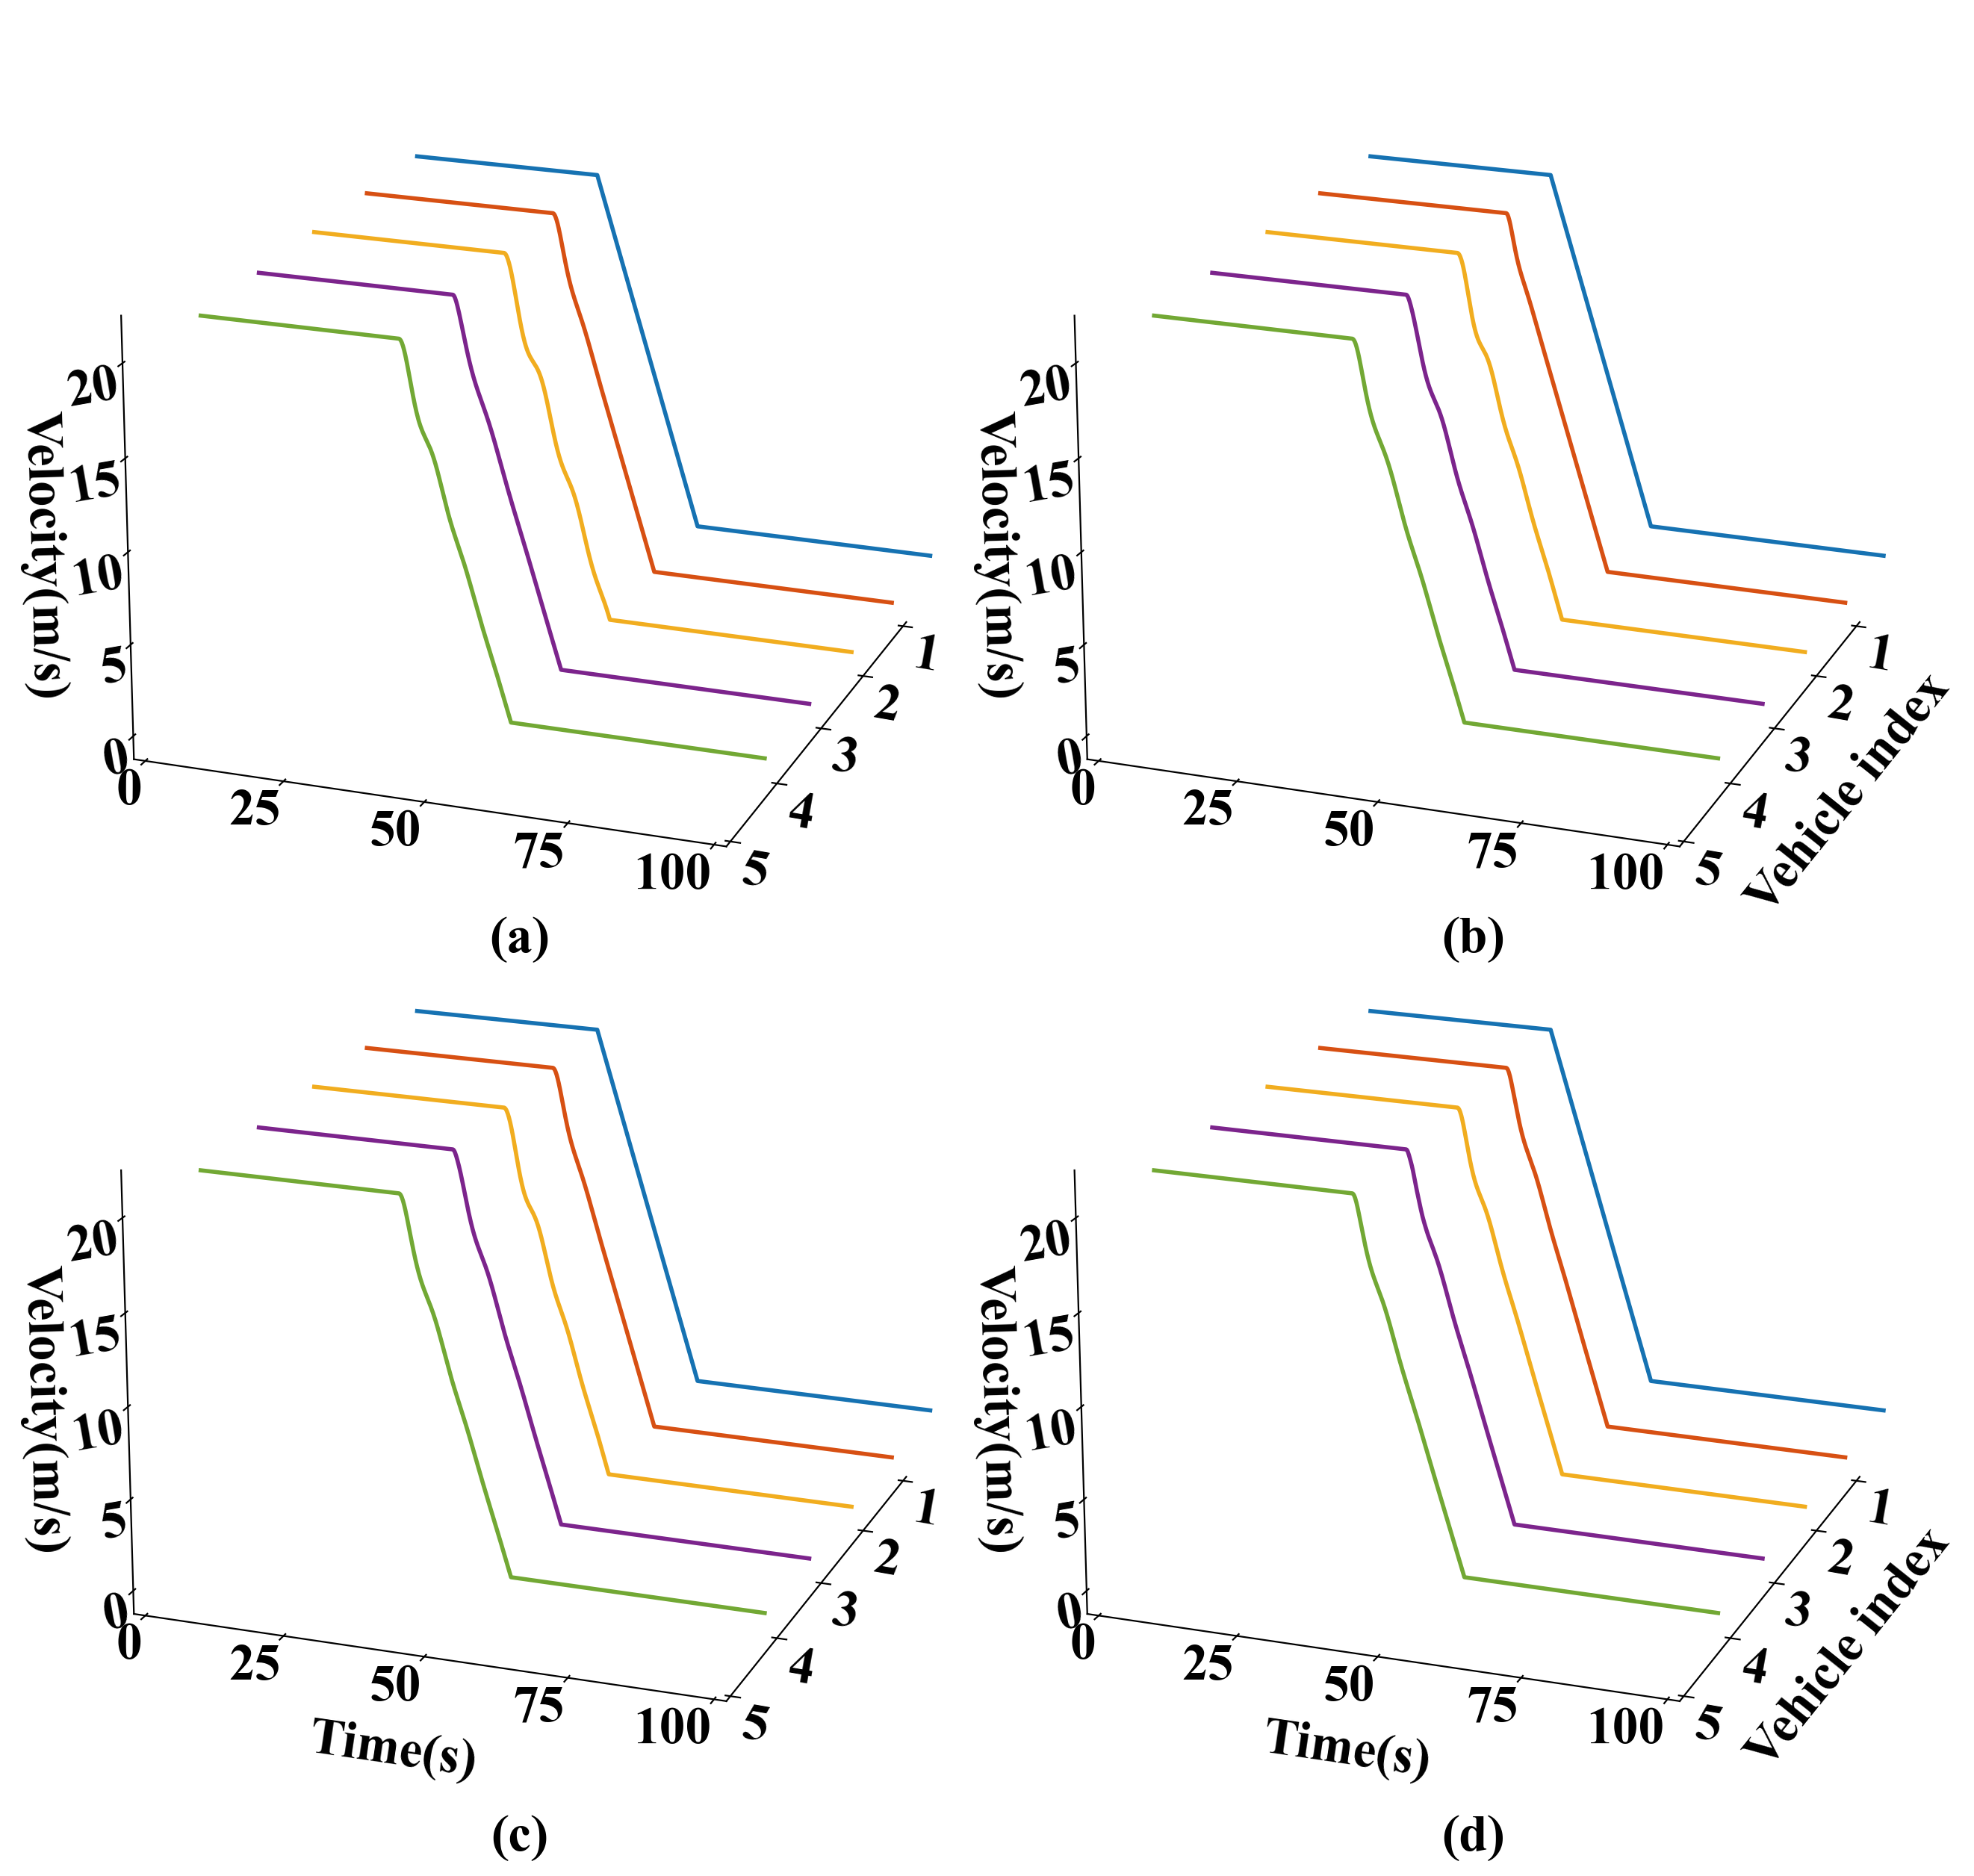
\includegraphics[width=14cm]{figs/fig6.png}
  \caption{~Tracking performance for a hard braking maneuver for each IFT under investigation: (a) LF; (b) LPF; (c) LMPF; (d) LBD.}
  \label{fig6}
\end{figure}

\begin{figure}
  \centering
  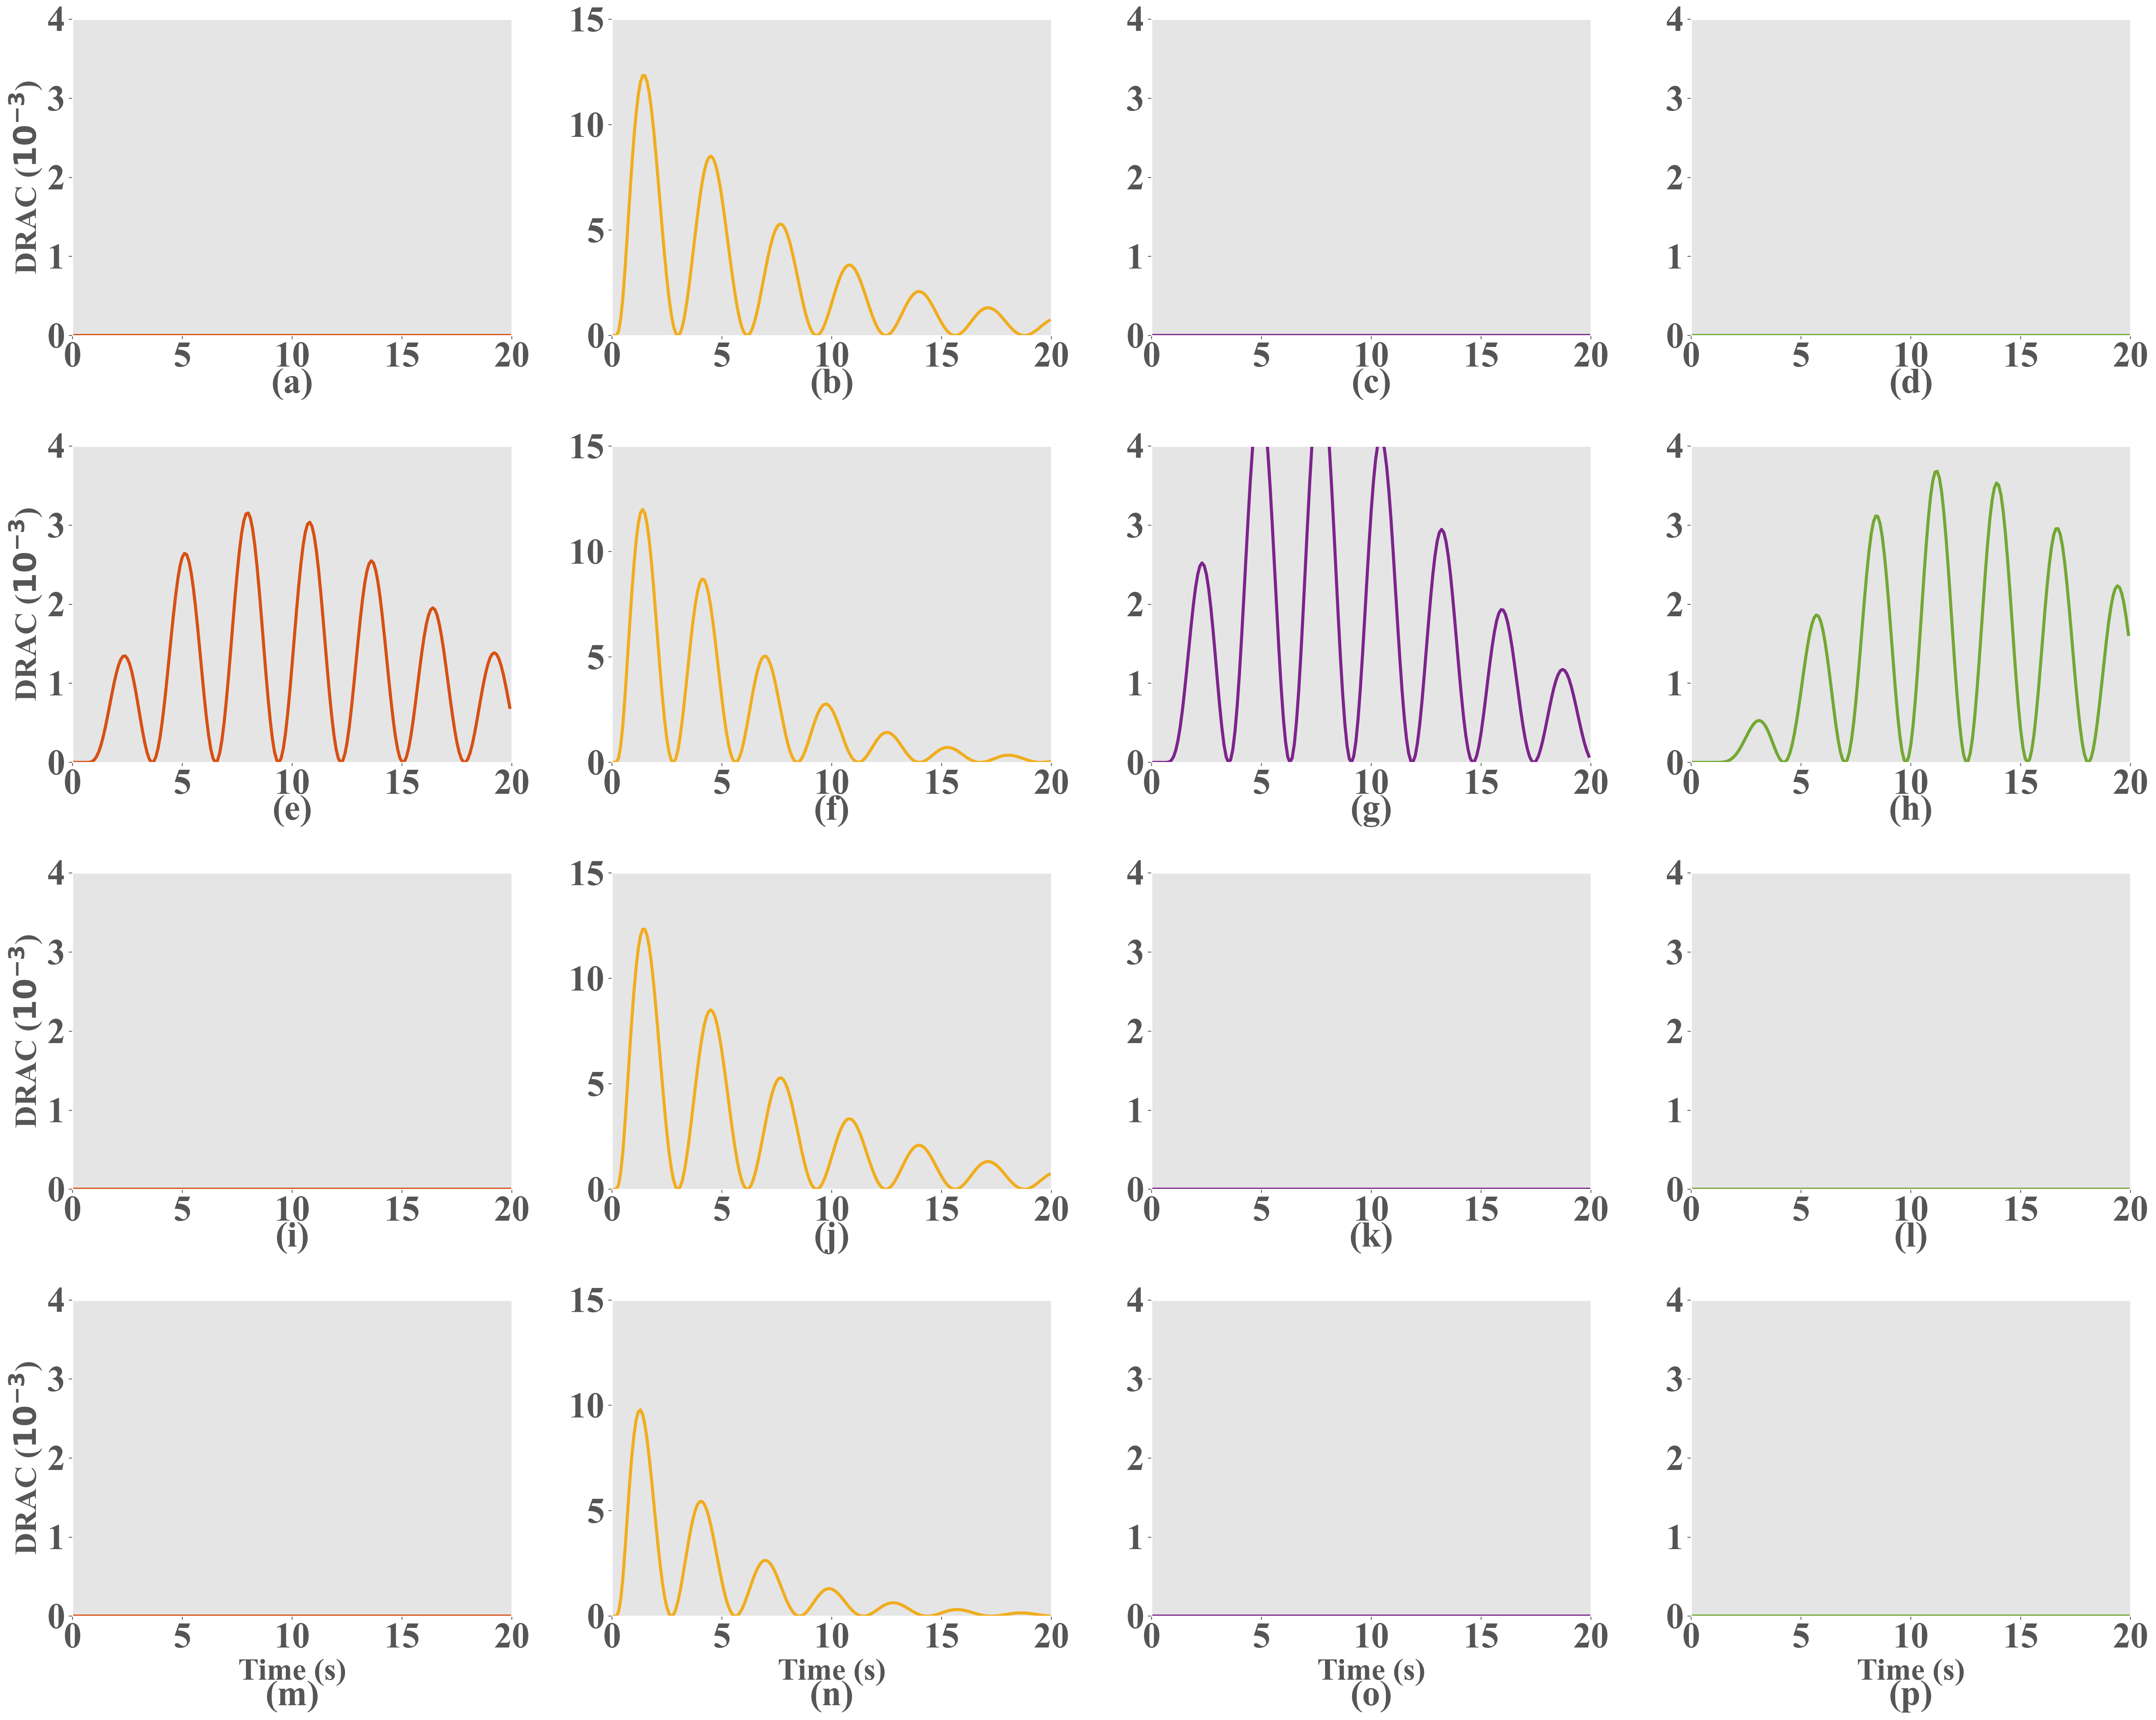
\includegraphics[width=14cm]{figs/fig7.png}
  \caption{~The DRAC variation of each CAV for each IFT under investigation: (a), (b), (c), and (d) present DRAC variation under LF of CAV2, CAV3, CAV4, CAV5, respectively; (e), (f), (g), and (h) show the case under LPF; (i), (j), (k), and (l) denote the case under LMPF; (m), (n), (o), and (p) show the case under LBD.}
  \label{fig7}
\end{figure}

From Fig.~\ref{fig7}, one phenomenon worth pointing out is that the CAV platoon is able to maintain a safety condition under hard braking maneuver. Since DRAC is less than 0.1 all-time, whatever Leader-based IFT and the control gain value under investigation are chosen. Moreover, from a vertical perspective, the case under LBD can provide better safety conditions than the other three one-direction communication IFTs. Besides, from a horizontal point of view, the choice of different control gains can significantly affect the variation of the safety indicator. The control gains of CAV3 are not conducive to safe driving due to its DRAC being significantly higher than other control gain schemes. Furthermore, different IFTs also affect the safety indicator. For example, the DRAC of CAV5 under LF is remarkably higher than that of CAV2 and CAV4. However, it can be kept low under the other three IFTs relative to the case under LF, since it can obtain more information to ensure safe driving. The case of CAV4 is quite the opposite, where the DRAC of CAV4 under LPF is significantly higher than the other three IFTs due to the additional poor information received from the immediate predecessor. In general, bi-direction communication and receiving more information in most cases enable a better safety condition for hard braking maneuver situations.


\section{Conclusion and future work}
\label{Section 6}

This paper proposed a general representation of the heterogeneous CAV platoon under the Leader-based IFT considering communication delay and engine actuator delay. To develop this general representation, graph theory was applied to depict communication within the CAV platoon under the Leader-based IFT, and a generic state model was established based on the dynamics of the closed-loop vehicular network. In addition, a novel and more unconservative stability condition of the CAV platoon was developed by applying the B-L inequalities and Lyapunov-Krasovskii Stability Theorem based on the general representation. Furthermore, a comprehensive performance evaluation analysis of the four typical Leader-based IFTs was conducted to reveal tracking performance, transient response, and safety conditions in various scenarios. Last but not least, this paper sheds some light on the relationship between safety conditions, control gains, and IFTs.

Admittedly, we acknowledge that the vehicle behavior is a simplified simulation of reality, and further field tests with more realistic vehicle dynamics models are needed. Moreover, this paper only deals with the case that adopts the CD policy while the Constant Time Headway policy is also widely adopted, which needs further investigation. Similarly, a more general IFTs need to be extended in further studies rather than only Leader-based IFTs. Another question to investigate further is that the communication delay adopted in this paper is the upper bound assumed to be constant for simplification. However, the communication delay is time-varying which changes with the surrounding environment. Future research is also needed toward developing a novel stability theorem to deal with time-varying communication delays.

\appendix


\section*{Appendix A.~Proof of Lemma~\ref{lemma5}}
\label{AppendixA}

Assume a function $x \in \mathcal{C}$, a matrix $R \in \mathbb{S}_n^ +  $, and $h > 0 $. Adopt the approximation error between $x(u) $ and its projection to the orthogonal sequence set $\left\{ {{\mathcal{L}_k},k \in \mathbb{N}} \right\} $ with respect to the inner product, which can be defined by:
\begin{equation}
  {y_N}\left( u \right) = x(u) - \sum\limits_{k = 0}^N {\frac{{\int_{ - h}^0 {{\mathcal{L}_k}} (u)x(u){\text{d}}u}}{{\int_{ - h}^0 {\mathcal{L}_k^2} (u){\text{d}}u}}} {\mathcal{L}_k}(u) = x\left( u \right) - \sum\limits_{k = 0}^N {\frac{{2k + 1}}{h}} {\Omega _k}{\mathcal{L}_k}(u)
  \label{eqapp1}
\end{equation}

Obviously, ${y_N} \in \mathcal{C}$ holds. Moreover, the integral $\int_{ - h}^0 {y_N^T} (u)R{y_N}(u){\text{d}}u$ exists and the orthogonal property (\ref{p3.1}) yields:
\begin{equation}
  \begin{gathered}
    \int_{ - h}^0 {y_N^T} (u)R{y_N}(u){\text{d}}u = \int_{ - h}^0 {{x^T}} (u)Rx(u){\text{d}}u \hfill \\
    \quad \quad \quad \quad \quad \quad \quad \quad  - 2\sum\limits_{k = 0}^N {\frac{{2k + 1}}{h}} {\left( {\int_{ - h}^0 {{\mathcal{L}_k}} (u)x(u){\text{d}}u} \right)^T}R{\Omega _k}(x) \hfill \\
    \quad \quad \quad \quad \quad \quad \quad \quad  + \sum\limits_{k = 0}^N {{{\left( {\frac{{2k + 1}}{h}} \right)}^2}} \left( {\int_{ - h}^0 {\mathcal{L}_k^2} (u){\text{d}}u} \right)\Omega _k^T(x)R{\Omega _k}(x). \hfill \\
  \end{gathered}
  \label{eqapp2}
\end{equation}

According to the definition, some derivation can be provided:
\begin{equation}
  \left\{ \begin{gathered}
    {\Omega _k}(x) = \int_{ - h}^0 {{\mathcal{L}_k}} (u)x(u){\text{d}}u \hfill \\
    {\left( {\frac{{2k + 1}}{h}} \right)^2}\int_{ - h}^0 {\mathcal{L}_k^2} (u)du = \frac{{2k + 1}}{h} \hfill \\
  \end{gathered}  \right.
  \label{eqapp3}
\end{equation}

Substituting the above Equation into Equation (\ref{eqapp2}), we get:
\begin{equation}
  \int_{ - h}^0 {y_N^T} (u)R{y_N}(u){\text{d}}u = \int_{ - h}^0 {{x^T}} (u)Rx(u){\text{d}}u - \sum\limits_{k = 0}^N {\frac{{2k + 1}}{h}} \Omega _k^T(x)R{\Omega _k}(x).
  \label{eqapp4}
\end{equation}

Moreover, the inequality (\ref{eqlemma5}) can be obtained by noting that $\int_{ - h}^0 {z_N^ \top } (u)R{z_N}(u){\text{d}}u > 0{\text{ }}$ for $R \succ 0$




\section*{Appendix B.~Feedback control for linearization}
\label{AppendixB}
In this appendix, we provide the linearization of the longitudinal vehicle dynamic in Equation (\ref{eq2}). The functions of the lumped uncertain resistance forces, including $f_i^g(t)$, $f_i^w(t)$, and $f_i^r(t)$ are expressed as follows:
\begin{equation}
  \left\{\begin{array}{l}
    f_{i}^{g}(t)=m_{i} g \sin \left(\theta_{i}(t)\right)                        \\
    f_{i}^{w}(t)=\frac{1}{2} \rho C_{D} A_{F}\left(v_{i}(t)+v_{w}(t)\right)^{2} \\
    f_{i}^{r}(t)=\mu_{R} m_{i} g \cos \left(\theta_{i}(t)\right)
  \end{array}\right.
  \label{eqapp5}
\end{equation}
where $g=9.81m/s^2$ denotes the acceleration of gravity; $\theta_i(t)$ is the inclination angle of the road; $\rho$ denotes the air density; $C_D$ is the aerodynamic drag coefficient; $A_F$ represents the maximal cross-sectional/frontal area of the vehicle; $v_w(t)$ denotes the uncertain headwind speed; $\mu_R$ is the coefficient of rolling resistance.

The desired engine dynamic is modeled as follows:
\begin{equation}
  (\tau_is+1)F_i^e=U_i
  \label{eqapp6}
\end{equation}

Adopting the inverse Laplace transformation on Equation (\ref{eqapp6}) arrives at:
\begin{equation}
  \dot{f_i^e}\left(t\right)=\frac{u_i(t)}{\tau_i}-\frac{f_i^e\left(t\right)}{\tau_i}
  \label{eqapp7}
\end{equation}

Substituting Equation (\ref{eq2}) into Equation (\ref{eqapp7}) and differentiating both sides of Equation (\ref{eqapp7}) with respect to time, we get:
\begin{equation}
  \begin{aligned}
    \dot{a}_{l}(t) & =\frac{\dot{f}_{l}^{e}(t)}{m_{i}}-\frac{\dot{f}_{l}^{g}(t)}{m_{i}}-\frac{f_{l}^{i \omega}(t)}{m_{i}}-\frac{\dot{f}_{l}^{r}(t)}{m_{i}}                                                                                         \\
                   & =               \frac{u_{i}(t)}{m_{i} \tau_{i}}                                                                                                                                                                               \\
                   & -               \frac{a_{i}(t)+\mathrm{g} \sin \left(\theta_{i}(t)\right)\left[1-\tau_{i} \mu_{R} \dot{\theta}_{l}(t)\right]+\mathrm{g} \cos \left(\theta_{i}(t)\right)\left[1+\tau_{i} \dot{\theta}_{l}(t)\right]}{\tau_{i}} \\
                   & -               \frac{\frac{1}{2} \rho C_{D} A_{F}\left(v_{i}(t)+v_{w}(t)\right)\left(\left(v_{i}(t)+v_{w}(t)\right)+2 \tau_{i}\left(a_{i}(t)+\dot{v}_{w}(t)\right)\right)}{\tau_{i}}
  \end{aligned}
  \label{eqapp8}
\end{equation}

Thus, the nonlinear state feedback chosen for linearizing can be defined by:
\begin{equation}
  \begin{aligned}
    u_i^\ast\left(t\right)= & m_iu_i\left(t\right)+g\sin{\left(\theta_i\left(t\right)\right)}\left[1-\tau_i\mu_R\dot{\theta_i}\left(t\right)\right]+g\cos{\left(\theta_i\left(t\right)\right)}\left[1+\tau_i\dot{\theta_i}\left(t\right)\right]\ \\
                            & +\frac{1}{2}\rho C_DA_F\left(v_i\left(t\right)+v_w\left(t\right)\right)\left(\left(v_i\left(t\right)+v_w\left(t\right)\right)+2\tau_i(a_i\left(t\right)+\dot{v_w}\left(t\right))\right)
  \end{aligned}
  \label{eqapp9}
\end{equation}

Under the new feedback control input, the Equation (\ref{eq2}) can be rewritten as:
\begin{equation}
  \tau_i\dot{a_i}\left(t\right)+a_i\left(t\right)=u_i(t)
  \label{eqapp10}
\end{equation}



\section*{Appendix C.~Proof of Corollary~\ref{corollary9}}
\label{AppendixC}
Applying Lemma~\ref{lemma5} to the order $N$, we get:
\begin{equation}
  \int_{ - h}^0 {{{\dot x}^T}} (u)R\dot x(u){\text{d}}u \geqslant \frac{1}{h}{\left[ {\begin{array}{*{20}{c}}
            {{\Omega _0}(\dot x)} \\
            {{\Omega _1}(\dot x)} \\
            \vdots                \\
            {{\Omega _N}(\dot x)}
          \end{array}} \right]^T}{R_N}\left[ {\begin{array}{*{20}{c}}
          {{\Omega _0}(\dot x)} \\
          {{\Omega _1}(\dot x)} \\
          \vdots                \\
          {{\Omega _N}(\dot x)}
        \end{array}} \right]
  \label{C1}
\end{equation}


An integration by parts of ${\Omega _k}(\dot x)$ ensures that, for all $k \geqslant 0$:
\begin{equation}
  {\Omega _k}(\dot x) = {\mathcal{L}_k}(0)x(0) - {\mathcal{L}_k}( - h)x( - h) - \int_{ - h}^0 {\left( {\frac{{\text{d}}}{{{\text{d}}u}}{\mathcal{L}_k}(u)} \right)} x(u){\text{d}}u
  \label{C2}
\end{equation}

Substituting the Boundary conditions (\ref{p3.2}) and Differentiation (\ref{p3.3}) into ${\Omega _k}(\dot x)$,we get:
\begin{equation}
  {\Omega _k}(\dot x) = x(0) - {( - 1)^k}x( - h) + \sum\limits_{i = 0}^{k - 1} {\frac{{\gamma _{Nk}^i}}{h}} {\Omega _i}(x) = {\Gamma _N}(k){\xi _N}
  \label{C3}
\end{equation}

Replacing ${\Omega _k}(\dot x)$ by ${\Gamma _N}(k){\xi _N}$ leads to Equation (\ref{eq18}).


\section*{Appendix D.~Proof of Theorem~\ref{theorem10}}
\label{AppendixD}
According to the Corollary~\ref{corollary9}, the states of system need to be extended to ${\tilde x_N}(t)$ defined as:
\begin{equation}
  {\tilde x_N}(t) = \left\{ \begin{gathered}
    \left[ {\begin{array}{*{20}{c}}
            {{x_t}(0)}                                               \\
            {\int_{ - h}^0 {{\mathcal{L}_0}} (s){x_t}(s){\text{d}}s} \\
            \vdots                                                   \\
            {\int_{ - h}^0 {{\mathcal{L}_{N - 1}}} (s){x_t}(s){\text{d}}s}
          \end{array}} \right] = \left[ {\begin{array}{*{20}{c}}
            {{x_t}(0)}                          \\
            {{\Omega _0}\left( {{x_t}} \right)} \\
            \vdots                              \\
            {{\Omega _{N - 1}}\left( {{x_t}} \right)}
          \end{array}} \right],\quad if\quad N \geqslant 1, \hfill \\
    {x_t}(0),\quad \quad \quad \quad \quad \quad \quad \quad \quad \quad \quad \quad if\quad N = 0. \hfill \\
  \end{gathered}  \right.
  \label{DX}
\end{equation}

The augmented vector ${\tilde x_N}(t) $ is composed by the instantaneous state ${x_t}(0) $ and the projections of the state function $ {x_t}$ to the $N $ first Legendre polynomials. According to Appendix C, an integration by parts allows expressing the time derivative of ${\tilde x_N}(t) $ as follows
\begin{equation}
  {\dot {\tilde x}_N}(t) = {H_N}{\xi _N}(t)
  \label{D1}
\end{equation}
where
\begin{equation}
  {\xi _N}(t) = \left\{ \begin{gathered}
    \left[ {\begin{array}{*{20}{c}}
            {x_t^T(0)}                                                          \\
            {x_t^T( - h)}                                                       \\
            {\frac{1}{h}\int_{ - h}^0 {{\mathcal{L}_0}} (s){x_t}(s){\text{d}}s} \\
            \vdots                                                              \\
            {\frac{1}{h}\int_{ - h}^0 {{\mathcal{L}_{N - 1}}} (s){x_t}(s){\text{d}}s}
          \end{array}} \right],\quad if\quad N \geqslant 1 \hfill \\
    \left[ {\begin{array}{*{20}{c}}
            {x_t^T(0)} \\
            {x_t^T( - h)}
          \end{array}} \right],\quad \quad \quad \quad \quad \quad if\quad N = 0 \hfill \\
  \end{gathered}  \right.
  \label{DX2}
\end{equation}

It is worth mentioning that states of the argument system are combined by states of the original delay system and of the Linear time-invariant (LTI) system. Moreover, there is only one delay term in Equation (\ref{D1}) is ${x_t}( - h)$. Therefore, the LKF can be chosen by:
\begin{equation}
  {V_N}\left( {{x_t},{{\dot x}_t}} \right) = \tilde x_N^T(t){P_N}{\tilde x_N}(t) + \int_{t - h}^t {{x^T}(s)Sx(s){\text{d}}s}  + h\int_{t - h}^t {\int_\theta ^t {{{\dot x}^T}(s)R\dot x(s){\text{d}}s{\text{d}}\theta } }
  \label{D2}
\end{equation}

Applying Lemma~\ref{lemma5} to Equation (\ref{D2}) yields:
\begin{equation}
  {V_N}\left( {{x_t},{{\dot x}_t}} \right) \geqslant \tilde x_N^T(t){\Theta _N}(h){\tilde x_N}(t) + h\int_{t - h}^t {\int_\theta ^t {{{\dot x}^T}(s)R\dot x(s){\text{d}}s{\text{d}}\theta } } \;
  \label{D3}
\end{equation}

The positive definiteness of $V_N$ is ensured by the condition $S \succ 0$, $R \succ 0$, and ${\Theta _N}(h) \succ 0$. Besides, ${\Theta _N}(h) \succ \left[ {\begin{array}{*{20}{c}}
          {{\varepsilon_1}I} & 0 \\
          0                  & 0
        \end{array}} \right]$ holds for a sufficiently small ${\varepsilon _1} > 0$ which implies that ${V_N}\left( {{x_t},{{\dot x}_t}} \right) \geqslant {\varepsilon _1}{\left| {{x_t}(0)} \right|^2}$. Furthermore, ${P_N} \prec \lambda \operatorname{diag} (I,I,3I,5I, \ldots ,(2N - 1)I)$ holds for a sufficiently large scalar $\lambda  > 0$. Therefore, it holds:
\begin{equation}
  \begin{gathered}
    {V_N}\left( {{x_t},{{\dot x}_t}} \right) \leqslant \lambda {\left| {{x_t}(0)} \right|^2} + \lambda \sum\limits_{i = 0}^{N - 1} {(2i + 1)} \Omega _i^T{\Omega _i} + \int_{t - h}^t {{x^T}} (s)Sx(s){\text{d}}s \hfill \\
    \quad \quad \quad \quad \quad  + h\int_{t - h}^t {\int_\theta ^t {{{\dot x}^T}(s)R\dot x(s){\text{d}}s{\text{d}}\theta } }  \hfill \\
  \end{gathered}
  \label{D4}
\end{equation}

According to Lemma~\ref{lemma5}, we get:
\begin{equation}
  \begin{gathered}
    {V_N}\left( {{x_t},{{\dot x}_t}} \right) \leqslant \lambda {\left| {{x_t}(0)} \right|^2} + \int_{t - h}^t {{x^T}(s)(\lambda hI + S)x(s){\text{d}}s}  \hfill \\
    \quad \quad \quad \quad \quad  + h\int_{t - h}^t {\int_\theta ^t {{{\dot x}^T}(s)R\dot x(s){\text{d}}s{\text{d}}\theta } }  \hfill \\
  \end{gathered}
  \label{D5}
\end{equation}
which guarantees that there exists a scalar ${\varepsilon _2} > 0$, such that ${V_N}\left( {{x_t},{{\dot x}_t}} \right) \leqslant {\varepsilon _2}\left| {{{\bar x}_t}} \right|_h^2$ holds for $\forall t > h$, where ${\bar x_t} = \left[ {\begin{array}{*{20}{c}}
          {{x_t}} \\
          {{{\dot x}_t}}
        \end{array}} \right]$. Then it holds:
\begin{equation}
  {\varepsilon _1}{\left| {{x_t}(0)} \right|^2} \leqslant {V_N}\left( {{x_t},{{\dot x}_t}} \right) \leqslant {\varepsilon _2}\left| {{{\bar x}_t}} \right|_h^2.
  \label{D6}
\end{equation}

After that, consider the derivative of $V_N$ for all $t \geqslant h$, we obtain:
\begin{equation}
  \begin{gathered}
    {{\dot V}_N}\left( {{x_t},{{\dot x}_t}} \right) = 2\tilde x_N^T(t){P_N}{{\dot \tilde x}_N}(t) + x_t^T(0)S{x_t}(0) \hfill \\
    \quad \quad \quad \quad  - x_t^T( - h)S{x_t}( - h) + {h^2}\dot x_t^T(0)R{{\dot x}_t}(0) \hfill \\
    \quad \quad \quad \quad  - h\int_{ - h}^0 {\dot x_t^T} (s)R{{\dot x}_t}(s){\text{d}}s. \hfill \\
  \end{gathered}
  \label{D7}
\end{equation}

Substituting ${\tilde x_N}(t) = {G_N}(h){\xi _N}(t)$, ${\dot {\tilde x}_N}(t) = {H_N}{\xi _N}(t)$, and ${\dot x_t}\left( 0 \right) = {F_N}{\xi _N}(t)$, we get:
\begin{equation}
  {\dot V_N}\left( {{x_t},{{\dot x}_t}} \right) = \xi _N^T(t){\Phi _{N0}}(h){\xi _N}(t) - h\int_{ - h}^0 {\dot x_t^T} (s)R{\dot x_t}(s){\text{d}}s
  \label{D8}
\end{equation}

Applying the Corollary~\ref{corollary9} to the order $N$ and injecting the resulting inequality (\ref{eq18}) into Equation (\ref{D8}) leads to:
\begin{equation}
  {\dot V_N}\left( {{x_t},{{\dot x}_t}} \right) \leqslant \xi _N^T(t){\Phi _N}(h){\xi _N}(t)
  \label{D9}
\end{equation}

Hence, if the LMIs (\ref{lmi22}) are satisfied, there exists a scalar ${\varepsilon _3} > 0$ such that ${\Phi _N}(h) \prec \left[ {\begin{array}{*{20}{c}}
          { - {\varepsilon _3}I} & 0 \\
          0                      & 0
        \end{array}} \right]$. Therefore, the following inequality holds:
\begin{equation}
  {\dot V_N}\left( {{x_t},{{\dot x}_t}} \right) \leqslant  - {\varepsilon _3}{\left| {{x_t}(0)} \right|^2},\quad \forall t \geqslant h
  \label{D10}
\end{equation}

The inequality (\ref{D10}) ensures the negative definiteness of ${\dot V_N}$. As for the stability of system (\ref{eq14}), by integrating inequality (\ref{D10}), we get:
\begin{equation}
  {V_N}\left( {{x_t},{{\dot x}_t}} \right) - {V_N}\left( {{x_h},{{\dot x}_h}} \right) \leqslant  - {\varepsilon _3}\int_h^t {{{\left| {{x_s}(0)} \right|}^2}} ds
  \label{D11}
\end{equation}
and, hence, Equation (\ref{D11}) yields:
\begin{equation}
  {\varepsilon _1}{\left| {{x_t}(0)} \right|^2} \leqslant {V_N}\left( {{x_t},{{\dot x}_t}} \right) \leqslant {V_N}\left( {{x_h},{{\dot x}_h}} \right) \leqslant {\varepsilon _2}\left| {{{\bar x}_h}} \right|_h^2
  \label{D12}
\end{equation}

Since ${\left| {{x_h}} \right|_h} \leqslant {c_1}|\phi {|_h}$, ${c_1} > 0$ \citep{Hale2013} and ${\left| {{{\dot x}_h}} \right|_h} \leqslant {c_2}|\phi {|_h}$, ${c_2} > 0$ according to the definition in Equation (\ref{eq14}), we obtain that:
\begin{equation}
  {\left| {{x_t}(0)} \right|^2} \leqslant \frac{{{V_N}\left( {{x_h},{{\dot x}_h}} \right)}}{{{\varepsilon _1}}} \leqslant {c_3}|\phi |_h^2,\quad {c_3} > 0
  \label{D13}
\end{equation}

Hence, system (\ref{eq14}) is stable. To prove asymptotic stability we note that, for any initial condition $\phi $, $x$ is uniformly continuous on $\left[ {0,\infty } \right)$ (since $x$ defined by the right-hand side of system (\ref{eq14}) is uniformly bounded). Moreover, Equation (\ref{D11}) yields that ${\left| {{x_t}(0)} \right|^2}$ is integrable on $\left[ {h,\infty } \right)$. Then, by Barbalat's lemma \citep{Min2007}, ${x_t}(0) \to 0$ as $t \to \infty $. Consequently, if the LMI of Theorem are satisfied, the delay system (\ref{eq14}) is asymptotically stable for the constant delay $h$.



% \afterpage{\clearpage}

\printcredits

\section*{Acknowledgment}

This research was sponsored by the National Science Foundation of China (No. 51878161 and No.52072067), Postgraduate Research \& Practice Innovation Program of Jiangsu Province (KYCX22\_0266), Natural Science Foundation of Jiangsu Province (No. BK20210249) and Jiangsu Planned Projects for Postdoctoral Research Funds (No. SBK2021041144).

%% Loading bibliography style file
% \bibliographystyle{model1-num-names}
\bibliographystyle{cas-model2-names}

% Loading bibliography database
\bibliography{cas-refs}


%\vskip3pt

\end{document}

